\begin{savequote}[9cm]
%Last night was a great night for the United States and for the world. A brutal killer, one who has caused so much hardship and death, has violently been eliminated. He will never again harm another innocent man, woman, or child. He died like a dog. He died like a coward. The world is now a much safer place.

Before 9/11, I am just a white guy, living a typical white guy's life. All my friends had names like Monica, Chandler, Joey, and Ross \dots I go to bed September tenth white, wake up September eleventh, I am an Arab.
\qauthor{--- Dean Obeidallah (as quoted in \citeauthor{Kundnani2014}, 2014, p. 51)}
\end{savequote}


\chapter[Does Terrorism Really Affect Attitudes?]{Does Terrorism Really Affect Attitudes?\footnote{This chapter is based on the following article:  Godefroidt, A. (n.d.). Does Terrorism Really Affect Citizens' Attitudes? A Meta-Analysis. \textit{Under Review.} This chapter and its corresponding working paper are, in turn, based on my thesis in the Master of Statistics, entitled ``A Three-Level Meta-Analysis of Terrorism and Social Cohesion: Do Terrorists Tear Us Apart?'' I would like to thank Prof. dr. Wim Van Den Noortgate for his supervision of this master thesis.}}
\chaptermark{Does Terrorism Really Affect Public Opinion?}
\label{chap:chap5}


\begin{chapabstract}
Does terrorism affect citizens’ political attitudes? If so, how and to what extent? This chapter performs a three-level meta-analysis of existing research on public reactions to terrorism, using a unique dataset of 1,709 effect sizes derived from 235 reports and over 400,000 respondents. The findings confirm that terrorism is associated—to a small but significant extent—with out-group hostility and political conservatism but not, as is often assumed, with unequivocal rally-‘round-the-flag effects. Here, the effects are predominantly driven by a post-9/11 rally-‘round-the-U.S.-flag effect. Furthermore, the review reveals important gaps and issues within this body of scholarship—most notably the absence of studies addressing non-Islamist violence or conducted in non-Western contexts. Taken together, this chapter contributes to ongoing debates about how the public reacts to terrorism which may help to counter potential democratic backlashes in times of terror.
\end{chapabstract}


%------------------------------------------------
\newpage
\section{Introduction}
%------------------------------------------------

Terrorist attacks often cause widespread concerns about possible implications of terrorism for core democratic values and ideals. For example, the recent series of terrorist attacks across Europe has been repeatedly associated with the steady rise of far-right and populist parties \citep{Fieschi2020}. Also, in France, several Muslim places of worship were blown up in revenge attacks following the Charlie Hebdo shootings \citep{Crone2015}. And the United Nations equally expressed concern about sharp increases in prejudice, racism, and xenophobia in the wake of 9/11 \citep{UNHCR2001}.


These concerns are well-justified based on previous studies on public reactions to terrorism. Overall, this literature seems to support the notion that terrorism, by triggering feelings of threat and injustice, evokes attitudinal reactions characterized by out-group hostility and in-group solidarity. More specifically, previous work has shown that terrorism, on the one hand, hardens people's attitudes towards out-groups in general and Muslims, Arabs, and immigrants in particular \citep[i.e., out-group hostility; see, e.g.,][]{Panagopoulos2006, Hopkins2010a, Echebarria-Echabe2009, Ferwerda2017}, increases support for more intrusive domestic and hawkish foreign policies \citep[e.g.,][]{Gadarian2010c, Davis2004, Fisk2019a}, and boosts the popularity of far-right and authoritarian political parties and politicians \citep[i.e., conservative shift; see, e.g.,][]{Vasilopoulos2019c, Nagoshi2008, Linden2018a, Marcus2019}. On the other hand, citizens also tend to turn inward following terrorist attacks by bolstering their attachment to and trust in the nation and its leaders \citep[i.e., rally-‘round-the-flag; see, e.g.,][]{VanHauwaert2020a, Dinesen2013a, Feinstein2018, Landau2004, Ladd2007, Lambert2010}. Over the past few decades, several cognitive and affective mediators have been suggested to explain this wide range of public reactions to terrorism \citep[e.g.,][]{Pyszczynski2003, Vasilopoulos2019c, Jost2019, Jost2017a, Marcus2019}.


Despite these valuable insights, our current understanding of how terrorism shapes social and political attitudes remains incomplete. First, to date, a systematic overview of how we have been studying this topic is still lacking. As a result, little is known about the signature features of this field of study. Second, the average strength of the relationship between terrorism and public attitudes remains unclear---which gives rise to conflicting narratives. While some authors worry that public reactions to terrorism put ``democracy at risk'' \citep{Merolla2009a}, others assert that such reactions are ``limited in size'' \citep{Sniderman2019a}, ``short-lived'' \citep{Arvanitidis2016}, or, in some cases, even non-existent \citep{Castanhosilva2018, Larsen2020}. Third, it remains unclear to what extent findings can be generalized across different research designs or, conversely, to what extent methodological decisions shape conclusions. By comprehensively comparing existing studies, this meta-analysis aims to generate insights into the precise ways in which terrorism is related to different social and political attitudes.


This study addresses these gaps by performing a systematic analysis of the research on terrorism and (1) out-group hostility, (2) political conservatism, and (3) rally-‘round-the-flag responses---using 1,709 effect sizes derived from 235 reports and covering over 400,000 respondents. First, key features of this particular field of study are identified, thereby revealing important empirical and methodological issues and gaps. Second, a preregistered three-level meta-analysis is performed to evaluate the existing empirical evidence for the out-group hostility, conservative shift, and rally-‘round-the-flag hypotheses. Third, a wide range of potential moderators are explored to assess whether and how the relationship between terrorism and attitudes is a function of particular research design features. Altogether, findings from this study contribute to the ever-growing literature on how violent incidents shape public opinion by suggesting promising avenues for future research, but they may equally inspire strategies and policies to counter potential democratic backlashes by providing a more nuanced understanding of when, why, and how the public reacts to terrorism. Before assessing the results of the review, theoretical foundations of the relationship between terrorism and sociopolitical attitudes are outlined (Section \ref{sec:52}) and the review protocol described (Section \ref{sec:53}).


\section{How Terrorism Affects Attitudes}
\label{sec:52}
For nearly a century, social scientists have attempted to understand why instances and periods of threat may affect citizens’ political and social ideas, attitudes, and behaviors. As a result, several theoretical perspectives have been used to explain public reactions to terrorism.\footnote{See Appendix \ref{app:A1} for the most commonly used theories in the field of terrorism effects studies.} These theories share two general assumptions. First, following cognitive dissonance theory \citep{Festinger1975}, they emphasize that situations can temporarily threaten one's sense of psychological security. Second, to cope with a collective and existential threat such as terrorism, people are expected to use coping mechanisms that transcend individual actions. Shifts in attitudes towards politics and other people are well-known collective coping mechanisms in times of terror \citep{Merolla2009a}. Yet, although most theories include elements of aversive arousal and collective coping, there are noteworthy differences between existing theories as to the centrality of cognitions versus emotions in inciting this arousal.


First, on a {cognitive} level, terrorism primes the unpredictability and inevitability of death \citep{Pyszczynski2003}, triggers the idea that oneself and one's country is in danger \citep{Jost2003, Huddy2002a}, and heightens perceptions of injustice and moral violations \citep{Lambert2019, Skitka2002}. At a more abstract level, terrorism thus challenges basic human assumptions about the world as being predictable, safe, and benign (Cannetti et al. \citeyear{Canetti2013a}, p. 267; see also shattered assumptions theory by Janoff-Bulman, \citeyear{Janoff-Bulman1992}). The {motivated social cognition} approach argues that, when confronted with ``a world that appears dangerous and unpredictable,'' people---even self-identified liberals---will adhere more strongly to ``conservative, authoritarian, and right-wing candidates, policies, and ideologies'' \citep[][pp. 326-327; see also Jost et al. \citeyear{Jost2003}]{Jost2017a}. Terror management theory, by contrast, asserts that, under life-threatening circumstances, people will strengthen their own worldviews---leading to political polarization instead of conservatism \citep{Pyszczynski2003}.


Second, on an {affective} level, terrorism is thought to elicit many forms of negative affect, including fear, anger, and sadness. One of the major advances in political psychology of the last decade, is the increased emphasis on specific or so-called 'discrete' emotions. While the dominant approach has long been to identify the unique roles played by positive versus negative affect in explaining human behavior, recent studies have demonstrated how discrete emotions of the same valence may entail different effects in the context of intergroup conflict \citep{Pliskin2020}. In the realm of terrorism studies, scholars have predominantly focused on the impact of fear and anger. In this respect, fearful individuals are shown to support more risk-aversive, defensive, and preventive actions \citep{Huddy2005, Lerner2003a, Skitka2006}, with feelings of anger and moral outrage being major drivers of support for more high-risk, punitive, and retributive actions \citep{Fisk2019a, Skitka2006, Wayne2018, Liberman2019a}.


It is, however, important to emphasize that attitudinal responses in times of terror will be jointly dependent on such cognitive and affective responses. Consistent with a standard dual-processing model, Sniderman and colleagues (\citeyear{Sniderman2019a}, p. 225) recently argued that emotional responses are automatically activated by terror attacks and can, with some effort, be subject to conscious control. Following classic appraisal theories, such conscious or cognitive reasoning might again feed emotions \citep{Moors2013}. In short, public reactions to terrorism are triggered by conscious and unconscious cognitions and emotions which are intertwined in a complex and circular way. 



Over the years, scholars have operationalized these responses in a myriad of ways. While some scholars have focused on increases in xenophobia, stereotypes, and prejudices to a wide range of out-groups \citep[e.g.,][]{Ferwerda2017, Choma2018, Maoz2008, Saleem2013}, others have assessed the relationship between terrorism and support for authoritarian, conservative, and right-wing policies and politicians \citep[e.g.,][]{Vasilopoulos2019c, Stroessner2015a, Brinson2012b}. Yet, still other studies, mainly situated within the rally-around-flag tradition, have documented surges in nationalism, patriotism, and political trust in the wake of an attack \citep[e.g.,][]{Feinstein2018, Ladd2007, Landau2004}. As a result, in this review, I follow these broader expectations in the literature by focusing on three clusters of outcomes, that is out-group hostility, political conservatism, and rally-‘round-the-flag responses in times of terror. More specifically, this meta-analysis assesses the empirical evidence for the following often-stated hypotheses in the literature: 


\vspace{2mm}
\noindent\textbf{H1.} Terrorism is positively associated with {out-group hostility.}

\vspace{2mm}
\noindent\textbf{H2.} Terrorism is positively associated with {political conservatism.}

\vspace{2mm}
\noindent\textbf{H3.} Terrorism is positively associated with {rally-‘round-the-flag} responses.



\section{Data and Methods}
In what follows, I outline the review protocol used to collect and analyze the existing empirical evidence for each of these hypotheses. This protocol was prepared according to the Preferred Studying Items for Systematic Reviews and Meta-Analyses Protocol \citep[PRISMA-P;][]{Shamseer2015} and was preregistered before data collection with PROSPERO International Prospective register of systematic reviews (\href{https://www.crd.york.ac.uk/prospero/display_record.php?RecordID=106160}{CRD42018106160}) and during data collection at osf.io (\href{https://www.osf.io/3jzs4}{osf.io/3jzs4}). More information the preregistration and deviations from it can be found in Appendix \ref{app:E1}.

\label{sec:53}
\subsection{Data}
\subsubsection{Data Collection}
A complementary four-step strategy was used to retrieve as many relevant studies as possible. First, several electronic databases were searched for relevant records using a broad search string.\footnote{Databases included in Web of Science (i.e., SSCI, A\&HCI, CPCI-SSH, BKCI-SSH), ProQuest (i.e., Criminal Justice Database, Political Science Database, Psychology Database, Social Science Database, Sociology Database, PsycARTICLES) and EBSCO (i.e., Criminal Justice Abstracts, OpenDissertations, Communication \& Mass Media Complete, ATLA Religion Database with ATLASerials PLUS) were used. The precise search term was: (prejudice OR stereotyp* OR out-group OR attitud* OR authoritarian* OR conservat* OR "public opinion" OR "policy support" OR "political consequences" OR "political tolerance" OR ideolog* OR voting OR vote*) AND (terror* OR attack* OR "political violence" OR bomb* OR "September 11" OR "9/11" OR "March 11" OR "Charlie Hebdo" OR "Paris attacks").} Second, a call for additional published or in-press articles, working papers, and unpublished data was put out on \href{https://twitter.com/AGodefroidt/status/1222913211512561665}{Twitter} and sent via the e-mail listservs of relevant societies in political science (i.e., the American Political Science Association, European Political Science Association, and European Consortium of Political Research), political psychology (i.e., International Society of Political Psychology), and terrorism studies (i.e., Society for Terrorism Research). I also personally contacted prominent scholars in the field with the same call for additional studies.\footnote{Importantly, I ensured to also contact scholars working on \textit{non}-Islamist (e.g., extreme right) terrorism as my search term predominately generated studies on unspecified or Islamist terrorism.} Third, the bibliography of relevant review articles were screened for additional citations (i.e., Ayer et al., 2017; Jost et al., 2017; Onraet et al., 2013; Sniderman et al., 2019).\footnote{These review articles are qualitative in nature or, when quantitative, did not perform a meta-analysis on the specific topic of this study.} Last, the references lists of all retrieved manuscripts were screened for additional citations, while the Social Sciences Citation Index was used to check on later citations of influential terrorism-effects studies. Using this comprehensive strategy, I identified 12,126 possibly relevant records. All these records were imported into Mendeley Reference Manager to check for and delete duplicate studies (n = 1,736 duplicates). The remaining 10,390 studies were screened for inclusion in the meta-analysis based on the following list of pre-defined inclusion and exclusion criteria:


%---------------------------------
% Table 1
%---------------------------------
\vspace{2mm}
\begin{table}[H]
\caption{Summary of Inclusion and Exclusion Criteria}
\label{tab:art4-tab1}
\small
\renewcommand{\arraystretch}{1.5} %spacing between rows
\begin{threeparttable}
\begin{tabular}{L{2cm}L{5.4cm}L{5.4cm}}
\hline
& \textbf{Inclusion criteria} & \textbf{Exclusion criteria} \\ \hline
Constructs & Studies on the relation between \textit{terrorism\tnote{a}} \hspace{2mm}and \textit{social and/or political attitudes\tnote{b}} & Studies on the impact of civil war, repression, genocide, random or non-political violence, or morality salience.  \\ 
Units & Studies with individuals as unit of analysis & Studies with communities, countries or other aggregated units of analysis. Studies using news articles, vote shares, tweets, etc. as their unit of analysis. \\ 
Study & English, French, and Dutch studies. No restriction regarding publication type or date.  & Studies in other languages \\
Designs & Studies reporting a quantitative measure of association and its precision between terrorism and sociopolitical attitudes & Systematic reviews and meta-analyses, focus groups, in-depth interviews, case reports, editorials, and commentaries \\
Statistics & Sufficient information to calculate effect sizes and precision & Insufficient information to calculate effect sizes and precision\tnote{c} \\ \hline
\end{tabular}
\begin{tablenotes}
\vspace{-5mm}
\singlespacing
\footnotesize
\item[a] Studies examining reactions to violence falling under the academic consensus definition of terrorism were eligible (Schmid, 2011) as well as studies that used terrorism as a label to describe one of their variables of interest. This two-folded strategy allowed to exhaustively take stock of how scholars in this field of research define and operationalize “terrorism.” 
\item[b] A broad operationalization of the outcome of interest was applied: \textit{Social attitudes} could include affective (e.g., feeling thermometers, out-group target emotions such as hatred/disgust/fear/anxiety or liking/warmth/sympathy/happiness), cognitive (e.g., beliefs, stereotypes, evaluations), behavioral (e.g., actual, intended, and self-reported actions toward out-group members such as helping, harming, social distance, avoidance) or policy-related (e.g., support for policies commonly associated with prejudice, such as immigration or confirmative action policies) attitudes towards an out-group. \textit{Political attitudes} could include measures of general political ideology (e.g., authoritarianism, social dominance orientation, general/social/economic conservatism, left-right/liberal-conservatism self-placement), nationalism (e.g., political and/or institutional trust, patriotism, national pride and identification), political participation (e.g., voting), and support for specific politicians or policies not related to an out-group (e.g., support for President Bush, domestic or foreign counter-terrorism measures).
\item[c] When studies did not report sufficient information, the corresponding author was contacted in order to obtain the necessary data. If the authors did not reply or supply this information after two reminders, the study was excluded from the meta-analysis. If, however, the (in)significance of the association was stated, a conservative approach was used by setting p-values $> \alpha$ to .90 and p-values $\leq \alpha$ to $\alpha$ .
\end{tablenotes}
\end{threeparttable}
\end{table}


Using these criteria, all studies were screened in two stages. In the first phase, a broad selection based on the title and abstract was performed, excluding research that clearly did not meet the selection criteria.\footnote{It is worth noting that the original corpus included numerous congressional reports, policy briefings, statements on votes and bills, presidential addresses, and news articles without any statistical information on the relationship of interest---hence, the large reduction in studies in this initial screening phase.} Next, the full text of the 943 remaining studies was retrieved and thoroughly screened to ascertain whether or not they met all inclusion and exclusion criteria. A final of 235 reports were withheld for analysis in this chapter. The PRISMA-flowchart in Figure \ref{fig:art4-fig1} summarizes the study selection process and includes an overview of the excluded studies as a function of the five criteria outlined above (based on the full-text screening, n = 943).

\vspace{3mm}
\begin{figure}[H]
\centering
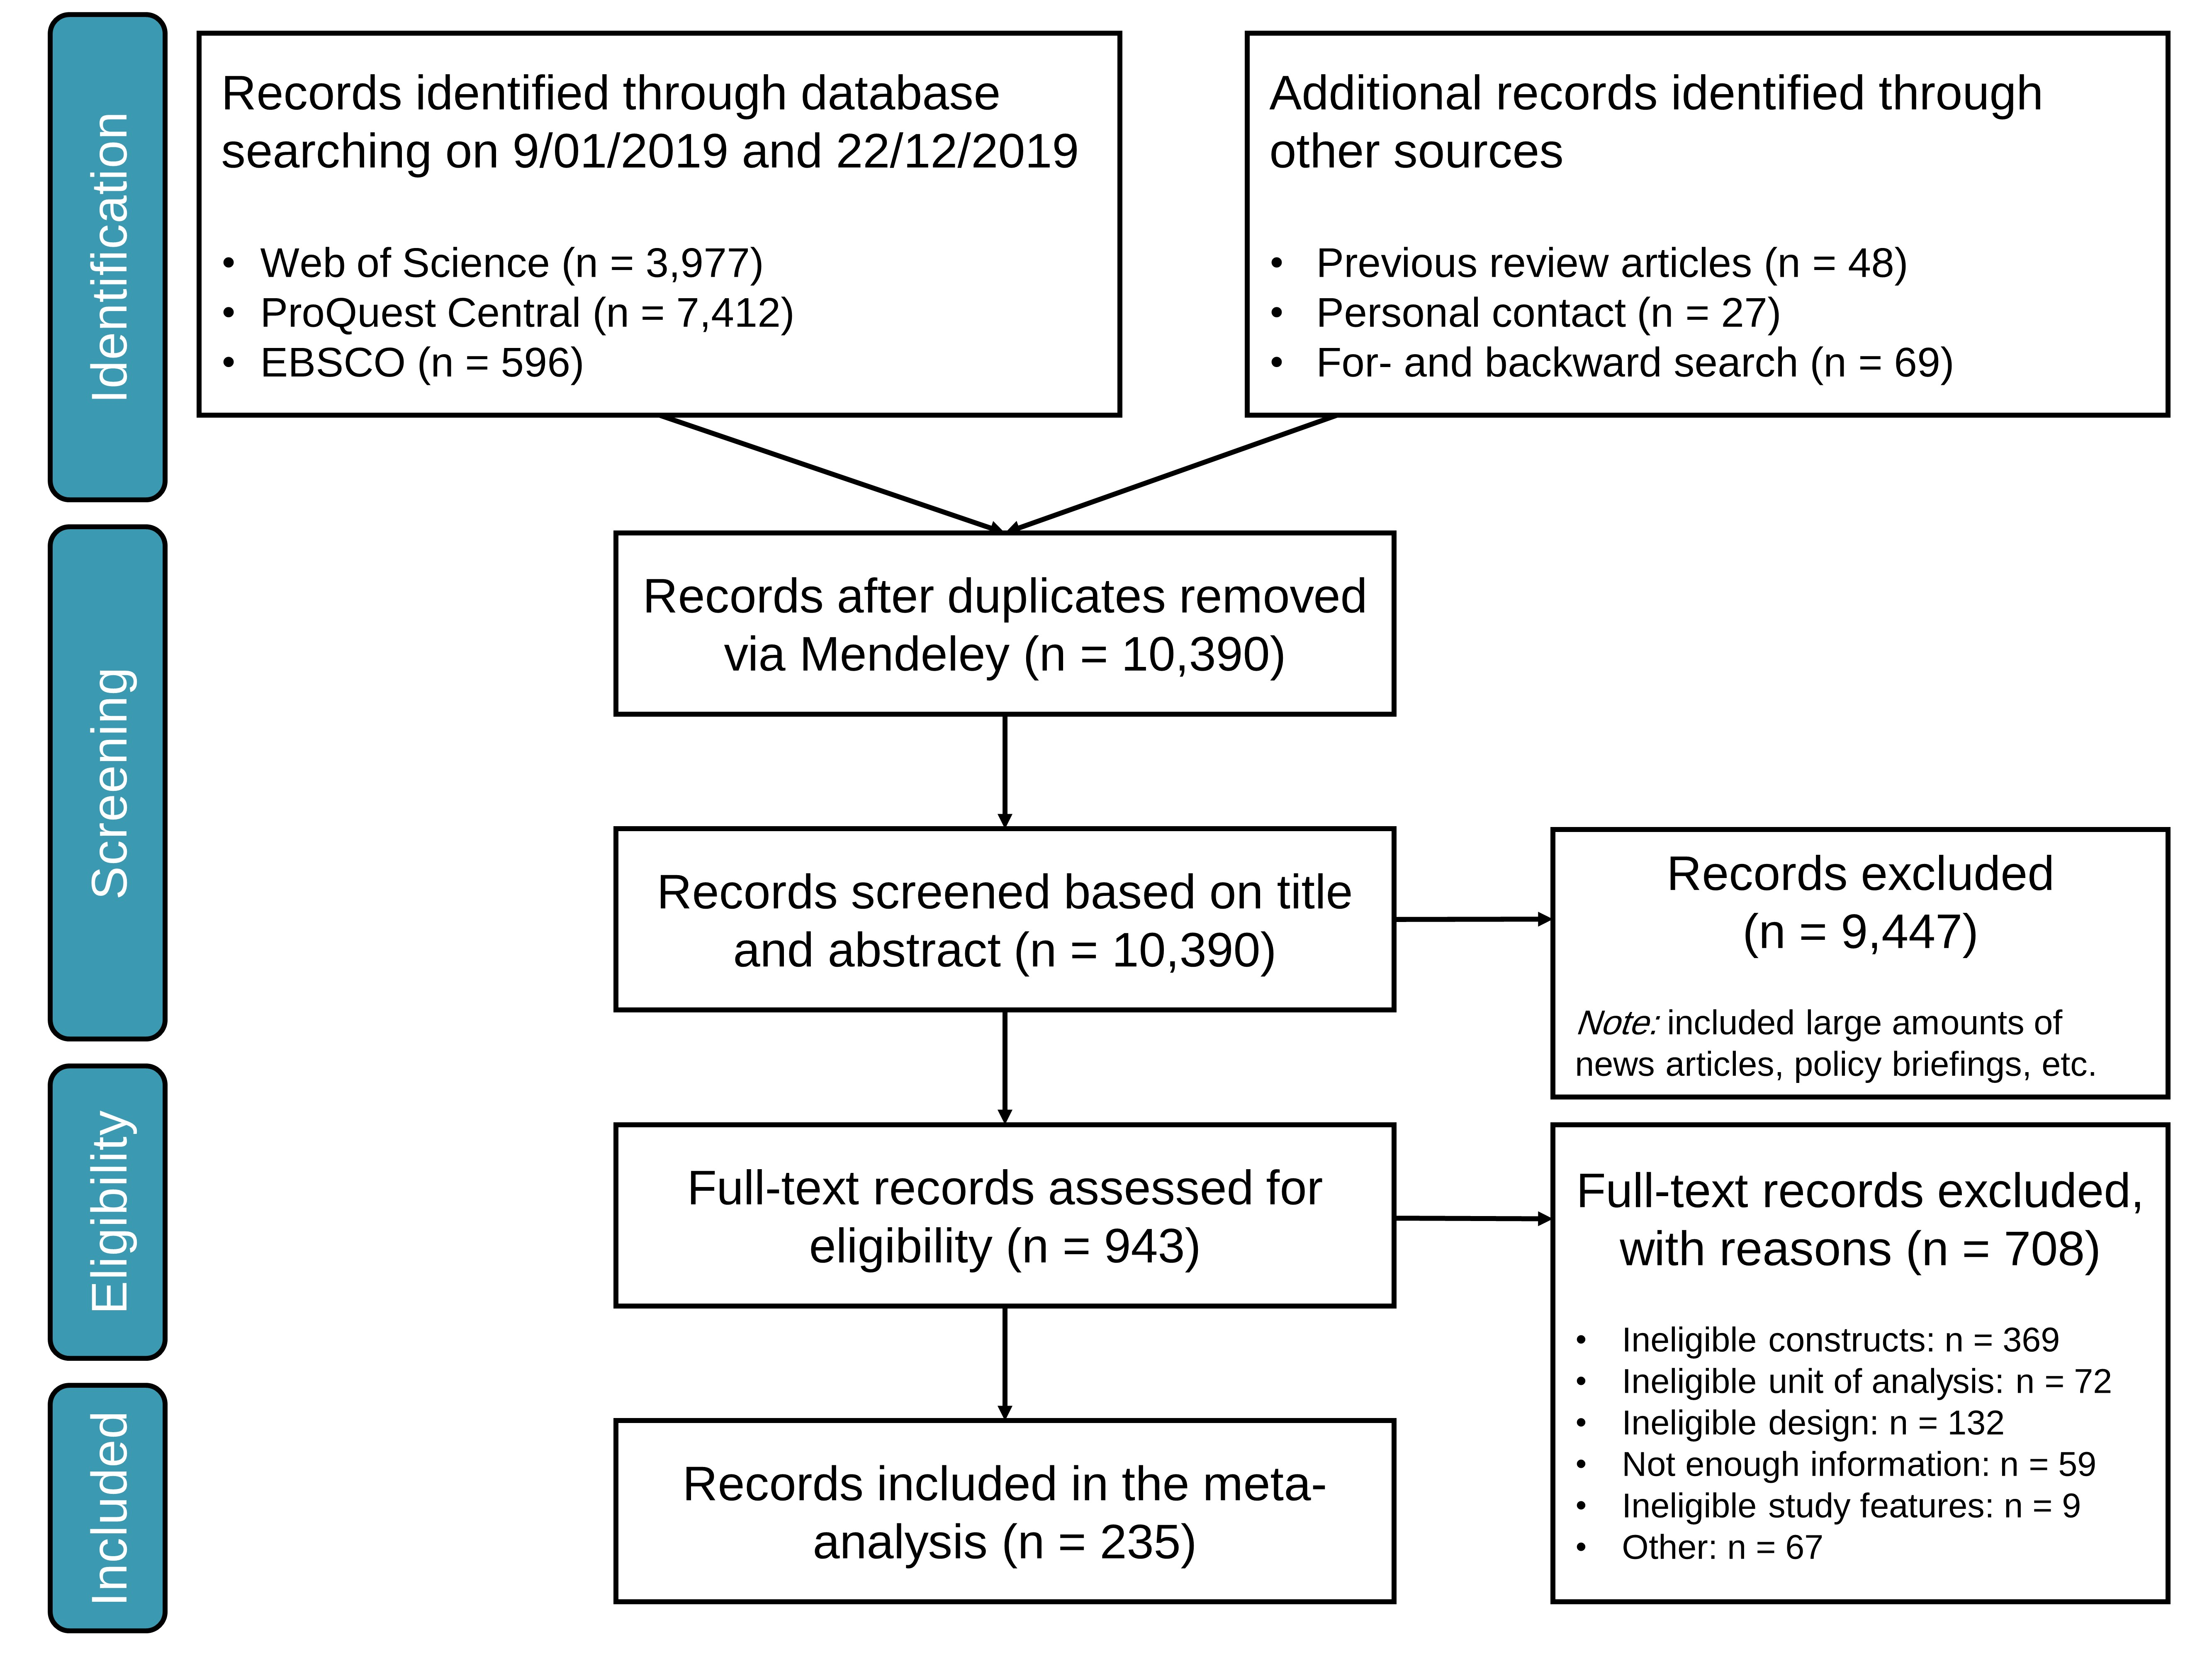
\includegraphics[width=\textwidth]{Chapter_5/art4-figure1.jpg}
\caption{PRISMA Flow Diagram of Selection Process}
\label{fig:art4-fig1}
\end{figure}
\vspace{3mm}



\subsubsection{Data Coding}
These 235 reports were then coded. Each reported association between terrorism and sociopolitical attitudes that met the selection criteria was coded as a separate case. A total of 1,709 associations were collected and coded. Based on a random selection of reports ($\pm$ 15\% of the final sample), the codebook to extract the necessary data was piloted and revised where necessary. The final codebook (see Appendix \ref{app:E2}) included six main categories of data. For each association, I extracted data related to the:

\begin{enumerate}[noitemsep]
    \item[(1)] report (including the authors, publication year, type of report, and publication status, impact factor if published, whether clear hypotheses were stated, \dots)
    \item[(2)] study (including whether the study employs data from an experiment, quasi-experiment, longitudinal study or survey, whether it was preregistered, \dots)
    \item[(3)] sample and its setting (including the country of study, sampling mechanism, response or attrition rate, mean age and gender distribution of the sample, \dots)
    \item[(4)] independent variable (including the exact measure of terrorism exposure, type/ideology of terrorism, casualty rate, \dots) 
    \item[(5)] dependent variable (including the exact type of outcome measure, whether it measures out-group hostility, political conservatism, or rally effects, and its reliability, whether there is a delay in-between the measurement of the IV and DV, \dots)
    \item[(6)] original test statistic and effect size(s)
\end{enumerate}


\subsubsection{Preparing Effect Sizes}
Because different studies (\textit{j} =1, 2, \dots, \textit{J}) used different ways to report the association (\textit{k} = 1, 2, \dots, \textit{K}) between terrorism and sociopolitical attitudes (e.g., correlation/regression coefficients, odds/risk ratios, mean differences etc.), each association was first converted into a Pearson’s correlation coefficient and calculated its corresponding sampling variance. Importantly, to meaningfully compare and pool effect sizes across studies, all correlations needed to reflect the relation between terrorism and sociopolitical attitudes in the same direction. Hence, where necessary, the direction of the correlation coefficient was changed, so that a positive value reflected an association between terrorism and higher levels of prejudice, xenophobia, conservatism, authoritarianism, political trust, nationalism, etc. Moreover, the sampling distribution of the correlation coefficient is skewed (i.e., non-normal) unless the population correlation is close to zero or unless the sample size is sufficiently large \citep{Cheung2015}. Therefore, a Fisher’s Z transformation was applied to approximate normally distributed effect sizes, by using the following formula:


\begin{equation}
y\textsubscript{z} = \frac{1}{2} \log\left(\frac{1 + r}{1 - r}\right).
\end{equation}


Last, univariate data were used as much as possible to calculate the common effect size. Studies only reporting multivariate regression coefficients are somewhat problematic as such coefficients represent partial correlation coefficients controlling for the influence of one or more covariates \citep{Peterson2005}. Hence, I first contacted the authors to solicit missing zero-order correlations but, if no such data could be extracted, I used the standardized ($\beta$) regression coefficient. Peterson and Brown (\citeyear{Peterson2005}) have shown that using beta coefficients to impute missing correlations generally produces relatively accurate and precise population effect-size estimates for meta-analyses using correlation coefficients as the effect-size metric. Potential benefits from applying this procedure include smaller sampling errors because of increased numbers of effect sizes and smaller non-sampling errors because of the inclusion of a broader array of research designs. 

\subsection{Methods}
\subsubsection{Three-Level Meta-Analysis and -Regressions}
\vspace{-2mm}
After calculating the common effect size and variance for each association $k$ in study $j$, a meta-analysis was performed to consolidate the overall strength of the association between terrorism and sociopolitical attitudes. To do so, a three-level random effects model was used. Raudenbush and Bryk (1985) showed how a meta-analysis can be considered a special case of multilevel models, except that aggregated instead of raw data are used. Traditional \textbf{two-level} random effects meta-analytic models assume that observed effect sizes differ because of (a) \textit{sampling error} (i.e., differences between observed effect sizes and population effects) and (b) \textit{between-study variance} (i.e., differences between the population effect sizes from different studies). 


However, the studies included in this meta-analysis reported 7.27 associations on average (SD = 8.24, range = $1-52$). This is predominantly because several measures of the same construct were used or several treatment groups were compared to a common control group. It is quite plausible that effect sizes from the same study are more similar than effect sizes from different studies. As a result, the important assumption of independent effect sizes underlying traditional random-effects models is likely to be violated. This is an important remark given that the vast majority of previous meta-analyses in the social sciences have opted to ignore dependence by including all effect sizes as if each effect size stems from an independent study \citep[e.g.,][]{Jost2017a} or to avoid dependence by either selecting one effect size per study or averaging effect sizes within studies \cite[e.g.,][]{Burke2013, Pettigrew2006}. However, because these approaches lead to incorrect estimations of the standard errors ($SE$s) of the parameter estimates and because they also reduce the research questions one can address, it is recommended to apply a third, but more complex, approach by modelling the dependent effect sizes \citep{VandenNoortgate2013}. Therefore, I performed a \textbf{three-level} meta-analysis that adds a third source of variance, namely (c) \textit{within-study/between-effect sizes variance} (i.e., differences between effect sizes coming from within the same study). Mathematically, the resulting model, in which studies are considered a random sample from the population of studies on terrorism and political attitudes, can be represented as follows:
\begin{equation}
y\textsubscript{kj} = \beta\textsubscript{0} + v\textsubscript{j} + u\textsubscript{kj} + e\textsubscript{kj}
\end{equation}

Thus, any observed effect size, $y_{kj}$, is assumed to be equal to an overall population effect size, $\beta_0$, plus a random deviation of the mean population effect size in study j from this overall population effect size, $v_j$, plus a random deviation of the k-th population effect size in study j from the mean effect in this particular study, $u_{kj}$, plus a random error deviation of the observed effect size from the population effect due to sampling fluctuation, $e_{kj}$. All three error terms are assumed to be independent and normally distributed with zero mean. Hence, the exact parameters estimated in this meta-analysis are the overall effect size, $\beta_0$, the between-study variance component, $\tau_{v}^2$, and the within-study variance component, $\tau_{u}^2$. Typically, the sampling variance, $\tau_{e}^2$, is not estimated but considered as known given that it can be derived based on the sample size for commonly used effect sizes measures. For a Fisher’s Z, as used in this meta-analysis, it has been shown that the sampling variance is equal to $\frac{1}{(n - 3)}$, with $n$ equal to the sample size.


In addition to correctly modeling the dependency in effect sizes, this three-level approach has the advantage that it allows to study the size of variation both between and within studies, and to look for moderator variables that explain part of this variation between and within studies. To that end, the model above can easily be extended by including characteristics of the studies (e.g., year or country of study), $x_j$, and of the effect sizes within studies (e.g., operationalization features), $x_{kj}$, as moderators:
\begin{equation}
y\textsubscript{kj} = \beta\textsubscript{0} +  \beta_1x\textsubscript{j} + \beta_2x\textsubscript{kj} + v\textsubscript{j} + u\textsubscript{kj} + e\textsubscript{kj}
\end{equation}


All meta-regressions used the maximum likelihood estimation procedure implemented in the {\ttfamily meta3} function from the {\ttfamily metaSEM} package in R. Importantly, out-group hostility, conservative shift, and rally-‘round-the-flag measures measures convey qualitatively different information about how the public responds to terrorism and, hence, cannot easily be aligned with each other. Therefore, the dataset was first split by hypothesis and three identical meta-analyses and quasi-identical meta-regressions were performed. This study contains 638 data points (from 123 reports) testing the out-group hostility hypothesis, 725 data points (from 142 reports) testing the conservative shift hypothesis, and 346 data points (from 68 reports) on the rally-‘round-the-flag hypothesis. Furthermore, for assessing moderator effects of categorical variables, one dummy indicator per category was included in the model and the intercept was constrained to zero. The advantage of this parameterization is that the regression coefficients can be interpreted as the average effect sizes for each category. Pairwise comparisons, using Benjamini-Hochberg correction for multiple testing, evaluated whether categories resulted in significantly different average effect sizes. When assessing moderator effects of continuous variables, the variables were centered around their mean to improve numerical stability and to facilitate interpretation of the intercept. After centering, the intercept denotes the predicted effect size when the moderator is at its mean value. 95\% Likelihood-based confidence intervals (LBCI) were used to test hypotheses on the parameter estimates as they are shown to be somewhat more accurate (see Cheung, 2015, pp. 30-34 for a comparison of the properties of Wald and Likelhood-based CIs.) Parameter estimates were considered significant when the LBCI did not include zero.



\subsubsection{Assessing Publication Bias}
One commonly acknowledged problem concerning meta-analyses is publication bias. In \citeyear{Begg1994}, Begg showed how significant results are more likely to be published than null results. As a result, meta-analyses—to a large extent relying on published studies—may overestimate the true mean effect size. Therefore, a number of graphical and statistical techniques were applied to assess and deal with publication bias (i.e., examining the moderating impact of publication status and sample size on the results, conducting Egger's regression tests, and constructing a funnel plot to visually detect publication bias). All these techniques rely in one way or another on the sample size as smaller studies require larger effect sizes to reach significance (see Appendix \ref{app:E3} for more information). 
\newpage

%One commonly acknowledged problem concerning meta-analyses is publication bias \citep{Begg1994}. In 1994, Begg showed how significant results are more likely to be published than null results. As a result, meta-analyses---to a large extent relying on published studies---may overestimate the true mean effect size. Therefore, I applied a number of graphical and statistical techniques to assess and deal with publication bias (i.e., examining the moderating impact of publication status and sample size on the results, conducting Egger's regression tests, and constructing a funnel plot to visually detect publication bias). All these techniques rely in one way or another on the sample size as smaller studies require larger effect sizes to reach significance \citep{Begg1994,VandenBussche2009}.


%\newpage

\section{Results}
\label{sec:54}
In what follows, the descriptive and inferential results of the review are reported. In line with the three gaps identified in the introduction, I begin by outlining key features of this field of study. Who is being studied, when and where do studies take place, how do the research designs look like, and what are commonly used treatments and measures? Second, I consolidate the overall effect sizes for the out-group hostility, conservative shift, and rally-‘round-the-flag hypotheses. Here, the degree of heterogeneity in effect sizes is quantified as well. In other words, I formally test whether there is variation in effect sizes between the studies included in this meta-analysis as well as between effect sizes within these studies. Last, I try to explain some of this heterogeneity between and within studies by adding Level-3 and Level-2 moderators for each of the three hypotheses central to this review.


\subsection{The Field Terrorism Effects Studies}
\label{sec:541}
What are the signature features of this field of study? Academic interest in the association between terrorism and public attitudes clearly commenced after the 9/11 attacks and was given an extra boost with the 2015-2016 ISIS attacks (fig. 5.2A/1B). Over the years (i.e., 1988-2020), exposure to terrorism has been operationalized in various ways (Table \ref{tab:art4-tab2}, fig. 5.2C). Sometimes participants were exposed to a news article or video clip about a particular act of violence, whereas at other times exposure happened more naturally when a terror attack occurred at the same time a survey was being fielded (acts of violence: 507 data points, 30\%). Sometimes studies gauged or manipulated citizens’ perception of the threat of terrorism (threat of violence: 520 data points, 30\%), while other studies were more interested in affective appraisals (fear: 146 data points, 9\%; anger: 111 data points, 6\%). And yet other studies asked respondents to report their own and/or relatives’ exposure to specific acts of violence (self-reported exposure: 184 data points, 11\%). 

The most frequently studied acts of violence are—perhaps unsurprisingly—9/11, the Israeli-Palestinian conflict, and 2015 series of ISIS attacks in Paris. Consequently, regarding the ideology behind the violence (fig. 5.2D), the vast majority of effect sizes quantify the effects of or relationship with Islamist terrorism (1046 data points, 61\%), whereas the share of information on how the public reacts to state terrorism (65 data points, 4\%) or extreme-right terror is remarkably low (35 data points, 2\%). It is interesting to note in this respect that only a handful of studies includes an explicit definition of ‘terrorism’—leading to the implicit assumption within this field of study that ‘terrorism’ is a clear-cut ‘you-know-it-when-you-see-it’ phenomenon. Furthermore, most studies are conducted in the United States (117 studies, 37\%), Israel (63 studies, 19\%), and Western European countries (112 studies, 35\%). Only seven studies (2\%) are conducted in non-Western contexts (i.e., two in Nigeria and one each in Egypt, Morocco, South-Africa, Colombia, and Pakistan).

In addition to a limited substantive and geographical scope, the review also reveals some important methodological gaps related to the research designs used. For instance, longitudinal studies are extremely rare (21 studies, 7\%), making it hard to assess the long-term impact of terrorism. Instead, almost half of the studies employ a cross-sectional design (152 studies, 48\%), with experiments and quasi-experiments used in 103 (32\%) and 41 (13\%) studies. Second, the mean statistical power across all studies included in this meta-analysis is 0.54 (SD = 0.37), which is below the generally accepted rule of $\geq$ 0.80. Hence, studies included in this body of scholarship tend to be underpowered, which increases the risk of both false negatives and false positives. Part of the explanation might be the fact that only ten studies (3\%) are reported as preregistered and, hence, conducted an a priori sample size calculation. In this respect, the median effective sample size is 301, with a minimum of 22 and a maximum of 37,670 participants (M = 1321.55, SD = 4209.84). 

Finally, the studies included in this meta-analysis are conducted among the general population (112 studies, 35\%), student samples (112 studies, 35\%), and other convenience samples (such as online opt-in panels, snowball samples, or online/social media samples; 93 studies, 29\%). The mean age across all samples is 33.23 years (SD = 11.48) and studies include 55\% women on average (SD = 13.71). Most studies examine the opinions of a majority group in the country of study (e.g., whites in the US, Israeli Jews in Israel; 135 studies, 42\%) or use a mixed sample (72 studies, 23\%). Only 15 studies (5\%) are conducted among participants of minority groups. The other 95 studies do not disclose information on the ethnic composition of their sample (30\%).


\begin{figure}[H]
\centering
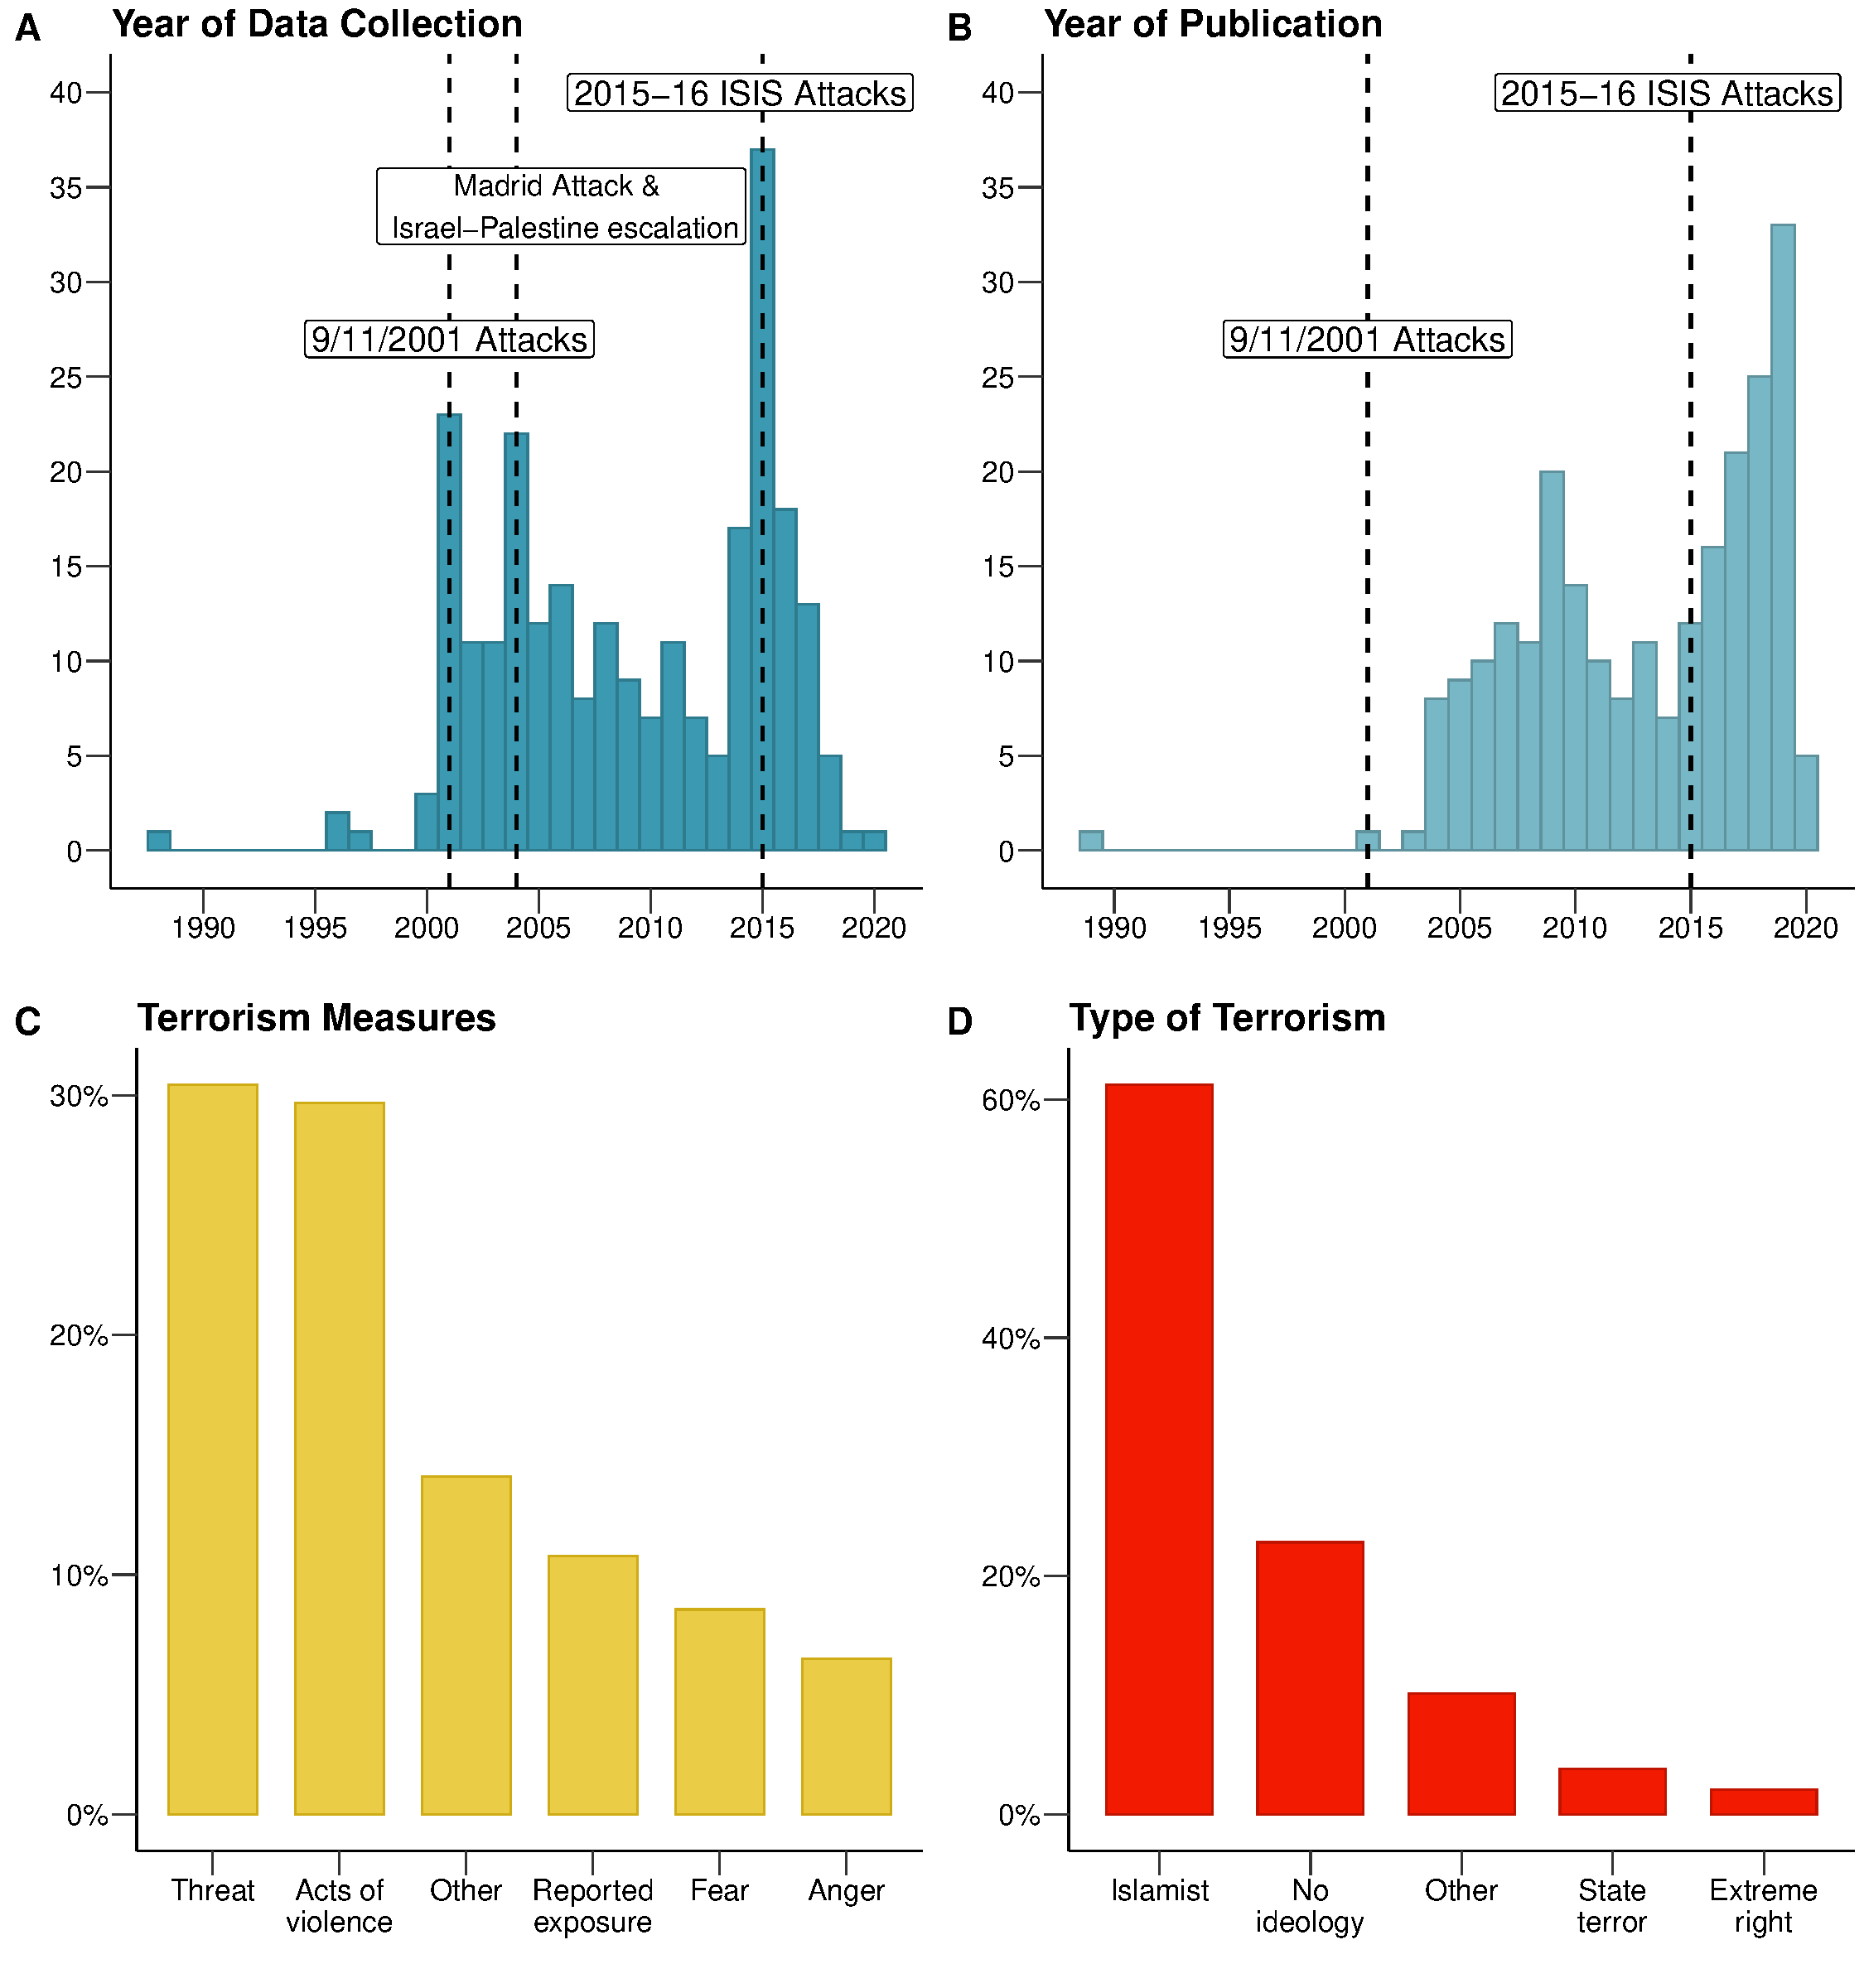
\includegraphics[width=\textwidth]{Chapter_5/art4-figure2.pdf}
\caption[Descriptives of Data Included in the Meta-Analysis]{\textbf{Descriptives of Data Included in the Meta-Analysis.} \textbf{(A)} Year the data was collected. \textbf{(B)} Year the report was published. \textbf{(C)} Main categories of terrorism measures used. \textbf{(D)} Main types/ideologies of terrorism studied.}
\label{fig:art4-fig2}
\end{figure}


\newpage
\begin{longtable}{@{}lp{10cm}@{}}
\caption{Measures and Manipulations Used to Gauge Citizens’ Exposure to or Appraisals of Terrorism}
\label{tab:art4-tab2}
\small \\
\toprule
Main category & Specific measures \\* \midrule
\endfirsthead
%
\multicolumn{2}{c}%
{{Table \thetable\ continued \dots}} \\
\toprule
Main category & Specific measures \\* \midrule
\endhead
\hline
\multicolumn{2}{r}{\textit{Continued on next page}} \\
\endfoot
\hline
\endlastfoot
%
Objective exposure & Pre- and post-violence measures \\
 & Days between act of violence and survey day \\
 & Newspaper vignette of act of violence \\
 & News clip of act of violence \\
 & Terrorism (vs., e.g., crime) wording of the questions \\
Self-reported exposure & Direct exposure to terrorism (e.g., witnessed, being injured) \\
 & Indirect exposure via friends and family \\
 & Indirect exposure via media reports \\
Cognitions & Self-reported concern/worry to become a victim of terrorism \\
 & Self-reported concern/worry for an attack on the nation \\
 & Manipulated vignette or writing task on the personal/national threat of terrorism \\
 & Manipulated percentage of the threat of terrorism \\
 & Remuneration of the threat of terrorism for oneself \\
Emotions & Anger/outrage (targeted at the phenomenon terrorism as such or at a particular attack or terrorist organization) \\
 & Fear/anxiety (idem) \\
 & Sadness (idem) \\
 & General negative valence (idem) \\
Other & Depression caused by terrorism \\
 & Post-Traumatic Stress Disorder caused by terrorism \\
 & Loss of resources (e.g., economic losses) \\* \bottomrule
\end{longtable}

\newpage
\subsection{Overall Effect Size and Effect Size Heterogeneity}
\label{sec:542}

To what extent is terrorism related to out-group hostility, political conservatism, or rally-‘round-the-flag responses? To answer this question, the dataset was split by hypothesis and the overall correlation coefficient was estimated based on an intercept-only three-level meta-analytic model for each of the hypotheses (see Materials and Methods for details). Table \ref{tab:art4-tab3} shows all overall estimated correlations (Zr), Likelihood-Based Confidence Intervals (LBCIs), number of correlations included (k), and heterogeneity indices. Note that all correlations are Fisher’s Z transformed. For ease of interpretation, however, the correlations mentioned in the text are backward transformed to their normal correlation scale (denoted as $\hat{\rho}$). 

Results show that terrorism is significantly associated with out-group hostility ($\hat{\rho}$ =.128), political conservatism ($\hat{\rho}$ = .132), and, to a lesser extent, rally-‘round-the-flag effects ($\hat{\rho}$ = .091). In other words, the more someone is exposed to, concerned about, or angry because of terrorism, the more he/she will derogate ‘others,’ find solace in conservative ideas, and bolster attachment to the nation and its leaders. At the same time, it is also important to note that all associations are fairly small \citep{Cohen1988}. 

\vspace{3mm}
\begin{table}[H]
\caption{Estimated Overall Fisher’s Z Effect Size, Likelihood-Based Confidence Intervals, and Heterogeneity Indices for All Three Hypotheses}
\label{tab:art4-tab3}
\begin{tabular}{@{}p{3cm}C{0.9cm}C{0.9cm}C{2.2cm}C{1cm}C{1cm}C{1cm}C{1cm}@{}}
\toprule
& $k$ & $Z_r$ & LBCI & $\tau_{(2)}^2$ & $\tau_{(3)}^2$ & $I_{(2)}^2$& $I_{(3)}^2$\\ \midrule
Outgroup Hostility & 638    & $.129$    & [$.096$; $.162$]  & $.009$ & $.030$ & $.221$ & $.752$\\
Conservative Shift & 725    & $.133$    & [$.109$; $.158$]  & $.009$ & $.017$ & $.333$ & $.628$\\
Rally Effects      & 346    & $.091$    & [$.054$; $.130$]  & $.009$ & $.019$ & $.314$ & $.667$\\ \bottomrule
\end{tabular}
\end{table}


Next, the heterogeneity variance estimates from the empty models (also Table \ref{tab:art4-tab2}) point to substantial differences in observed effect sizes both within and between studies for all three clusters of outcome measures. Indeed, likelihood ratio tests confirm that significant difference are found between effect sizes within studies for the out-group hostility [$\chi^2(1)$=400.148, p < .001], conservative shift [$\chi^2(1)$=253.054, p < .001], and rally effects [$\chi^2(1)$=128.502, p < .001] measures. In addition, significant differences are found between studies for all three hypotheses [$\chi^2(1)$=8102.953, p < .001 for out-group hostility; $\chi^2(1)$=9032.076, p < .001 for conservative shift; and $\chi^2(1)$=7594.119, p < .001 for rally effects]. 


\newpage
\subsection{Moderation Analyses} 
\label{sec:543}

To what extent are these differences in observed effect sizes, both between studies and between effect sizes within studies, explained by various moderating variables? In what follows, I provide a short description of the significant moderators for each of the hypotheses, whereas the exact estimates of the corresponding meta-regression models are available in Table \ref{tab:art4-tab4} for the out-group hostility hypothesis, Table \ref{tab:art4-tab5} for the conservative shift hypothesis, and Table \ref{tab:art4-tab6} for the rally-‘round-the-flag hypothesis. 


\subsubsection{Out-Group Hostility}
First, several features of the independent variable impact the observed effect size quantifying the relationship between terrorism and out-group hostility. For example, in addition to a dearth of research on non-Islamist terrorism, those few studies looking at non-Islamist terrorism also result in a significantly weaker, and even non-significant, overall effect size. Specifically, the average correlation coefficient for studies on Islamist terrorism and out-group attitudes is .124, compared to only .058 for studies looking at non-Islamist terrorism. Additionally, more objective measures of exposure to acts of violence (such as experiments or quasi-experiments) lead to significantly a lower average correlation, compared to other ways of measuring the independent variable (see Table \ref{tab:art4-tab4} for all coefficients as well as pairwise comparisons). 


Similarly, characteristics of the dependent variable influence the results. For example, the target out-group under scrutiny shows a significant main effect. More specifically, although terrorism is associated with significant increases in hostility towards all out-groups studied, the average effect size is about twice the size when examining attitudes towards religious out-groups and immigrants/refugees, than towards other out-groups. In addition, the data also support a so-called ‘guilt-by-association’ effect. That is, the average correlation equals .157 when there is a strong association between the perpetrator of the attack (e.g., an Islamist organization) and the out-group under scrutiny (e.g., Muslims), .106 when there is a weak association (e.g., Islamist terrorism and immigrants/refugees as out-group), and .089 when there is no such association (e.g., unspecified terrorism and immigrants/refugees as out-group). 


Finally, several methodological factors equally affect the observed effect size. Notably, the findings indicate that correlational studies result in higher effect sizes, compared to both experiments and quasi-experimental and longitudinal studies. In a similar vein, the mean effect size is significantly lower when there is at least one day between the measurement of the independent (e.g., the terrorist attack or experimental manipulation) and dependent variable. Second, student samples result in a lower average correlation, compared to general population samples and, particularly, other convenience samples. As a result, the mean age in the samples used is also a significant predictor of the strength of the relationship between terrorism and out-group hostility. Last, while studies conducted in the United States and Israel display similar average effect sizes, studies conducted outside these contexts result in a significantly lower average correlation. 

\vspace{3mm}
\begin{ThreePartTable}
\setlength{\tabcolsep}{4.5pt}
\begin{TableNotes}
\vspace{-4mm}
\footnotesize
\singlespacing
\item\textit{Note}: $k$ = number of effect sizes in the category. $b$ = unstandardized regression coefficient. The regression coefficients for the categorical variables can be interpreted as the mean effect size (i.e. Fisher’s Z correlation coefficient) for each category. Effect sizes belonging to one categorical variable that do not share subscripts differ at $p < .05$ after Benjamini-Hochberg correction for multiple comparisons. LBCI = Likelihood-Based Confidence Interval. LRT = Likelihood Ratio Test. $R^2$ refers to the proportion of the explained total variance across the levels.
\end{TableNotes}
\begin{longtable}[c]{llcrrcc}
\caption[Moderator Analyses for Out-Group Hostility Hypothesis]{\textbf{Moderator Analyses for Out-Group Hostility Hypothesis.} \\\textbf{(PANEL A)} Models as a Function of Characteristics of the Independent Variables. \\\textbf{(PANEL B)} Models as a Function of Characteristics of the Dependent Variable. \\\textbf{(PANEL C) }Models as a Function of Sample and Study Characteristics.}
\label{tab:art4-tab4} \\
\toprule
\multicolumn{7}{l}{\textbf{PANEL A. CHARACTERISTICS OF THE INDEPENDENT VARIABLE}} \\
\hline
\endfirsthead
%
\multicolumn{7}{c}%
{{Table \thetable\ continued \dots}} \\
\hline
\endhead
%
\hline
\multicolumn{7}{r}{\textit{Continued on next page}} \\
\endfoot
\hline
\insertTableNotes  % tell LaTeX where to insert the contents of "TableNotes"
\endlastfoot
%
\multicolumn{2}{l}{{Moderator}} & \multicolumn{1}{c}{{$k$}} & \multicolumn{1}{c}{{$b$}} & \multicolumn{1}{c}{{95\% LBCI}} & \multicolumn{1}{c}{{$R^2$}} & \multicolumn{1}{c}{{LRT Statistic}} \\ \hline
\multicolumn{2}{l}{Ideology} & 638 &  &  & .033 & $\chi^2(2)=8.783, p=.012$ \\
 & Islamist\textsubscript{a,b} & 466 & .124 & [.089, .160] &  &  \\
 & Non-Islamist\textsubscript{a} & 113 & .058 & [-.011, .126] &  &  \\
 & No ideology\textsubscript{b} & 59 & .180 & [.127, .232] &  &  \\
\multicolumn{2}{l}{Measurement} & 638 &  &  & .126 & $\chi^2(4)= 34.464, p<.001$ \\
 & Obj. exposure\textsubscript{a} & 247 & .045 & [-.005, .094] &  &  \\
 & Subj. exposure\textsubscript{a} & 65 & .111 & [.060, .161] &  &  \\
 & Cognitions (threat)\textsubscript{b} & 153 & .211 & [.167, .256] &  &  \\
 & Emotions (anger, fear)\textsubscript{b,c} & 72 & .189 & [.138, .240] &  &  \\
 & Residual category\textsubscript{a,c} & 101 & .145 & [.095, .195] &  &  \\ [1.5ex] \hline
 \multicolumn{7}{l}{\textbf{PANEL B. CHARACTERISTICS OF THE DEPENDENT VARIABLE}} \\ \hline
 \multicolumn{2}{l}{{Moderator}} & \multicolumn{1}{c}{{$k$}} & \multicolumn{1}{c}{{$b$}} & \multicolumn{1}{c}{{95\% LBCI}} & \multicolumn{1}{c}{{$R^2$}} & \multicolumn{1}{c}{{LRT Statistic}} \\ \hline
\multicolumn{2}{l}{Target out-group} & 638 &  &  & .045 & $\chi^2(2)= 11.536, p=.003$ \\
 & Religious\textsubscript{a} & 327 & .146 & [.109, .183] &  &  \\
 & Immigrant/refugee\textsubscript{a} & 207 & .132 & [.090, .174] &  &  \\
 & Other out-group\textsubscript{b} & 104 & .076 & [.029, .122] &  &  \\
\multicolumn{2}{l}{Guilt-by-association} & 638 &  &  & .059 & $\chi^2(2)=16.593, p<.001$ \\
 & Strong association\textsubscript{a} & 293 & .158 & [.122, .194] &  &  \\
 & Weak association\textsubscript{b} & 156 & .107 & [.065, .149] &  &  \\
 & No association\textsubscript{b} & 189 & .089 & [.048, .130] &  & \\ [1.5ex] \hline
 \multicolumn{7}{l}{\textbf{PANEL C. CHARACTERISTICS OF THE SAMPLE AND STUDY}} \\ \hline
 \multicolumn{2}{l}{{Moderator}} & \multicolumn{1}{c}{{$k$}} & \multicolumn{1}{c}{{$b$}} & \multicolumn{1}{c}{{95\% LBCI}} & \multicolumn{1}{c}{{$R^2$}} & \multicolumn{1}{c}{{LRT Statistic}} \\ \hline
\multicolumn{2}{l}{Research design} & 638 &  &  & .091 & $\chi^2(2)=9.691, p=.008$ \\
 & Experimental\textsubscript{a} & 141 & .092 & [.034, .150] &  &  \\
 & Correlational\textsubscript{b} & 283 & .169 & [.128, .210] &  &  \\
 & Other\textsubscript{a} & 214 & .092 & [.041, .144] &  &  \\
\multicolumn{2}{l}{Interval between IV-DV} & 638 &  &  & .053 & $\chi^2(1)=7.989, p=.005$ \\
 & Yes: interval\textsubscript{a} & 188 & .063 & [.007, .119] &  &  \\
 & No: direct\textsubscript{b} & 450 & .145 & [.111, .180] &  &  \\
\multicolumn{2}{l}{Sampling protocol} & 638 &  &  & .112 & $\chi^2(2)=29.050, p<.001$ \\
 & General population\textsubscript{a} & 200 & .157 & [.104, .210] &  &  \\
 & Student sample\textsubscript{b} & 273 & .058 & [.012, .104] &  &  \\
 & Convenience sample\textsubscript{a} & 165 & .192 & [.143, .241] &  &  \\
\multicolumn{2}{l}{Country} & 638 &  &  & .039 & $\chi^2(2)=6.900, p=.032$ \\
 & U.S.\textsubscript{a} & 159 & .169 & [.117, .221] &  &  \\
 & Israel\textsubscript{a,b} & 160 & .162 & [.085, .238] &  &  \\
 & Other\textsubscript{b} & 319 & .086 & [.041, .132] &  &  \\
\multicolumn{2}{l}{Mean age} & 545 & .004 & [.085, .162] & .087 &  \\
\multicolumn{2}{l}{Percentage women} & 591 & .001 & [-.000, .003] & .020 &  \\
\multicolumn{2}{l}{Data collection year} & 544 & -.002 & [-.008, .003] & .002 &  \\
\multicolumn{2}{l}{Publication year} & 638 & -.009 & [-.008, .006] & .000 & $\chi^2(1)=0.075, p=.784$ \\* \bottomrule
\end{longtable}
\end{ThreePartTable}
\newpage

\subsubsection{Conservative Shift}

As with the results for the out-group hostility hypothesis, the overall effect size for those few studies examining non-Islamist terrorism is significantly lower, compared to studies assessing the impact of Islamist or unspecified terrorism. Second, the exact measurement or manipulation used to gauge terrorism exposure also moderates the effect sizes. Again, studies using more objective measures of terrorism exposure (e.g., experiments and quasi-experiments) result in the lowest overall effect size, whereas studies using cognitive threat perceptions or affective appraisals result in significantly higher effect sizes.

There is considerable variation in average correlations depending on the exact operationalization of the outcome variable. More specifically, the highest effect sizes are found for studies examining changes in right-wing authoritarianism or in support for stricter security policies at the expense of civil liberties, whereas a lower effect size is found in studies looking at social dominance orientation. A residual category comprising measures of, for example, help for terrorism victims and more liberal environmental policies fails to reach statistical significance. All pairwise comparisons (with Benjamini-Hochberg correction for multiple testing) can be found in Table \ref{tab:art4-tab5}.

Finally, the results for the conservative shift hypotheses are slightly more consistent across research design features. For example, contrary to the out-group hostility literature, neither the country of a study nor a delay between the measurement of the dependent and independent variable significantly affects the overall effect size. However, in keeping with the results of the out-group hostility hypothesis, correlational studies and studies using convenience samples result in significantly higher overall effect sizes.

\vspace{3mm}

\begin{ThreePartTable}
\setlength{\tabcolsep}{4.5pt}
\begin{TableNotes}
\vspace{-4mm}
\footnotesize
\singlespacing
\item\textit{Note}: $k$ = number of effect sizes in the category. $b$ = unstandardized regression coefficient. The regression coefficients for the categorical variables can be interpreted as the mean effect size (i.e. Fisher’s Z correlation coefficient) for each category. Effect sizes belonging to one categorical variable that do not share subscripts differ at $p < .05$ after Benjamini-Hochberg correction for multiple comparisons. LBCI = Likelihood-Based Confidence Interval. LRT = Likelihood Ratio Test. $R^2$ refers to the proportion of the explained total variance across the levels.
\end{TableNotes}
\begin{longtable}[c]{llcrrcc}
\caption[Moderator Analyses for Conservative Shift Hypothesis]{\textbf{Moderator Analyses for Conservative Shift Hypothesis.} \\\textbf{(PANEL A)} Models as a Function of Characteristics of the Independent Variables. \\\textbf{(PANEL B)} Models as a Function of Characteristics of the Dependent Variable. \\\textbf{(PANEL C) }Models as a Function of Sample and Study Characteristics.}
\label{tab:art4-tab5}
\small \\
\toprule
\multicolumn{7}{l}{\textbf{PANEL A. CHARACTERISTICS OF THE INDEPENDENT VARIABLE}} \\
\hline
\endfirsthead
%
\multicolumn{7}{c}%
{{Table \thetable\ continued \dots}} \\
\hline
\endhead
%
\hline
\multicolumn{7}{r}{\textit{Continued on next page}} \\
\endfoot
\hline
\insertTableNotes  % tell LaTeX where to insert the contents of "TableNotes"
\endlastfoot
%
\multicolumn{2}{l}{{Moderator}} & \multicolumn{1}{c}{{$k$}} & \multicolumn{1}{c}{{$b$}} & \multicolumn{1}{c}{{95\% LBCI}} & \multicolumn{1}{c}{{$R^2$}} & \multicolumn{1}{c}{{LRT Statistic}} \\ \hline
\multicolumn{2}{l}{Ideology} & 725 &  &  & .080 & $\chi^2(2)=8.214, p=.016$ \\
 & Islamist\textsubscript{a} & 398 & .132 & [.104, .161] &  &  \\
 & Non-Islamist\textsubscript{b} & 191 & .075 & [.027, .124] &  &  \\
 & No ideology\textsubscript{a} & 136 & .159 & [.125, .192] &  &  \\
\multicolumn{2}{l}{Measurement} & 638 &  &  & .164 & $\chi^2(2)=26.425, p<.001$ \\
 & Obj. exposure\textsubscript{a} & 152 & .075 & [.035, .115] &  &  \\
 & Subj. exposure\textsubscript{a} & 95 & .106 & [.062, .150] &  &  \\
 & Cognitions (threat)\textsubscript{b} & 248 & .160 & [.130, .189] &  &  \\
 & Emotions (anger, fear)\textsubscript{b} & 128 & .181 & [.144, .218] &  &  \\
 & Residual category\textsubscript{a} & 102 & .102 & [.062, .143] &  & \\ [1.5ex] \hline
 \multicolumn{7}{l}{\textbf{PANEL B. CHARACTERISTICS OF THE DEPENDENT VARIABLE}} \\ \hline
 \multicolumn{2}{l}{{Moderator}} & \multicolumn{1}{c}{{$k$}} & \multicolumn{1}{c}{{$b$}} & \multicolumn{1}{c}{{95\% LBCI}} & \multicolumn{1}{c}{{$R^2$}} & \multicolumn{1}{c}{{LRT Statistic}} \\ \hline
\multicolumn{2}{l}{Outcome measure} & 725 &  &  & .089 & $\chi^2(5)=36.584, p<.001$ \\
 & RWA\textsubscript{a} & 75 & .173 & [.134, .211] &  &  \\
 & SDO\textsubscript{b} & 46 & .107 & [.060, .153] &  &  \\
 & Ideology\textsubscript{b} & 120 & .114 & [.080, .149] &  &  \\
 & Military actions\textsubscript{a,b} & 290 & .139 & [.109, .169] &  &  \\
 & Civil liberties\textsubscript{a} & 143 & .167 & [.132,  .203] &  &  \\
 & Residual category\textsubscript{c} & 51 & .005 & [-.055, .064] &  & \\ [1.5ex] \hline
 \multicolumn{7}{l}{\textbf{PANEL C. CHARACTERISTICS OF THE SAMPLE AND STUDY}} \\ \hline
 \multicolumn{2}{l}{{Moderator}} & \multicolumn{1}{c}{{$k$}} & \multicolumn{1}{c}{{$b$}} & \multicolumn{1}{c}{{95\% LBCI}} & \multicolumn{1}{c}{{$R^2$}} & \multicolumn{1}{c}{{LRT Statistic}} \\ \hline
\multicolumn{2}{l}{Research design} & 725 &  &  & .091 & $\chi^2(2)=12.946, p=.002$ \\
 & Experimental\textsubscript{a} & 199 & .100 & [.063, .137] &  &  \\
 & Correlational\textsubscript{b} & 417 & .160 & [.133, .188] &  &  \\
 & Other\textsubscript{a} & 109 & .092 & [.051, .133] &  &  \\
\multicolumn{2}{l}{Interval between IV-DV} & 725 &  &  & .033 & $\chi^2(1)=2.930, p=.087$ \\
 & Yes: interval\textsubscript{a} & 76 & .089 & [.033, .145] &  &  \\
 & No: direct\textsubscript{a} & 649 & .138 & [.114, .163] &  &  \\
\multicolumn{2}{l}{Sampling protocol} & 725 &  &  & .024 & $\chi^2(2)=8.626, p=.013$ \\
 & General population\textsubscript{a} & 263 & .105 & [.070, .140] &  &  \\
 & Student sample\textsubscript{a} & 224 & .127 & [.089, .164] &  &  \\
 & Convenience sampleb & 238 & .181 & [.140, .223] &  &  \\
\multicolumn{2}{l}{Country} & 725 &  &  & .023 & $\chi^2(2)=2.571, p=.277$ \\
 & U.S.\textsubscript{a} & 276 & .149 & [.114, .184] &  &  \\
 & Israel\textsubscript{a} & 202 & .140 & [.091, .190] &  &  \\
 & Other\textsubscript{a} & 247 & .111 & [.075, .148] &  &  \\
\multicolumn{2}{l}{Mean age} & 600 & .001 & [-.000, .003] & .014 &  \\
\multicolumn{2}{l}{Percentage women} & 657 & .000 & [-.001, .001] & .001 &  \\
\multicolumn{2}{l}{Data collection year} & 605 & -.002 & [-.006, .002] & .024 &  \\
\multicolumn{2}{l}{Publication year} & 725 & -.003 & [-.008, .001] & .019 & $\chi^2(1)=2.247, p=.133$ \\* \bottomrule
\end{longtable}
\end{ThreePartTable}

\vspace{3mm}


\subsubsection{Rally-‘Round-the-Flag}

While rally effects are fairly consistent across different methodological and substantive features, the significant moderators suggest that rally effects are primarily driven by a post-9/11 rally-‘round-the-US-flag effect or by an even more idiosyncratic rally-‘round President Bush effect. First and foremost, only studies conducted in the United States result in a statistically significant and substantial overall effect size of .158. In contrast, studies conducted in Israel result in an insignificant effect of .004 and studies conducted in yet other settings result in a statistically significant but negligible effect of .051. It is also important to note in this respect about 30 percent of the effect sizes come from U.S.-based studies, 15 percent from Israeli-based studies, and the other 55 percent of the effect sizes are scattered across 22 countries. 

Furthermore, as Figure \ref{fig:art4-fig3}A shows, the effect sizes decrease over time, with a particularly strong overall effect size of .224 found for those studies explicitly referring to 9/11. Figure \ref{fig:art4-fig3}B, in turn, shows that studies on non-Islamic terrorism result in a lower and statically insignificant average correlation, yet this comparison fails to reach significance due to the dominance of studies on Islamist terrorism within this sub-field of research. Finally, studies examining rallies around Republican politicians, incumbents, and, particularly, around President Bush result in significantly higher effect sizes. For all meta-regression estimates related to studies on rally effects, see Table \ref{tab:art4-tab6} below.

\newpage

\begin{figure}[H]
\centering
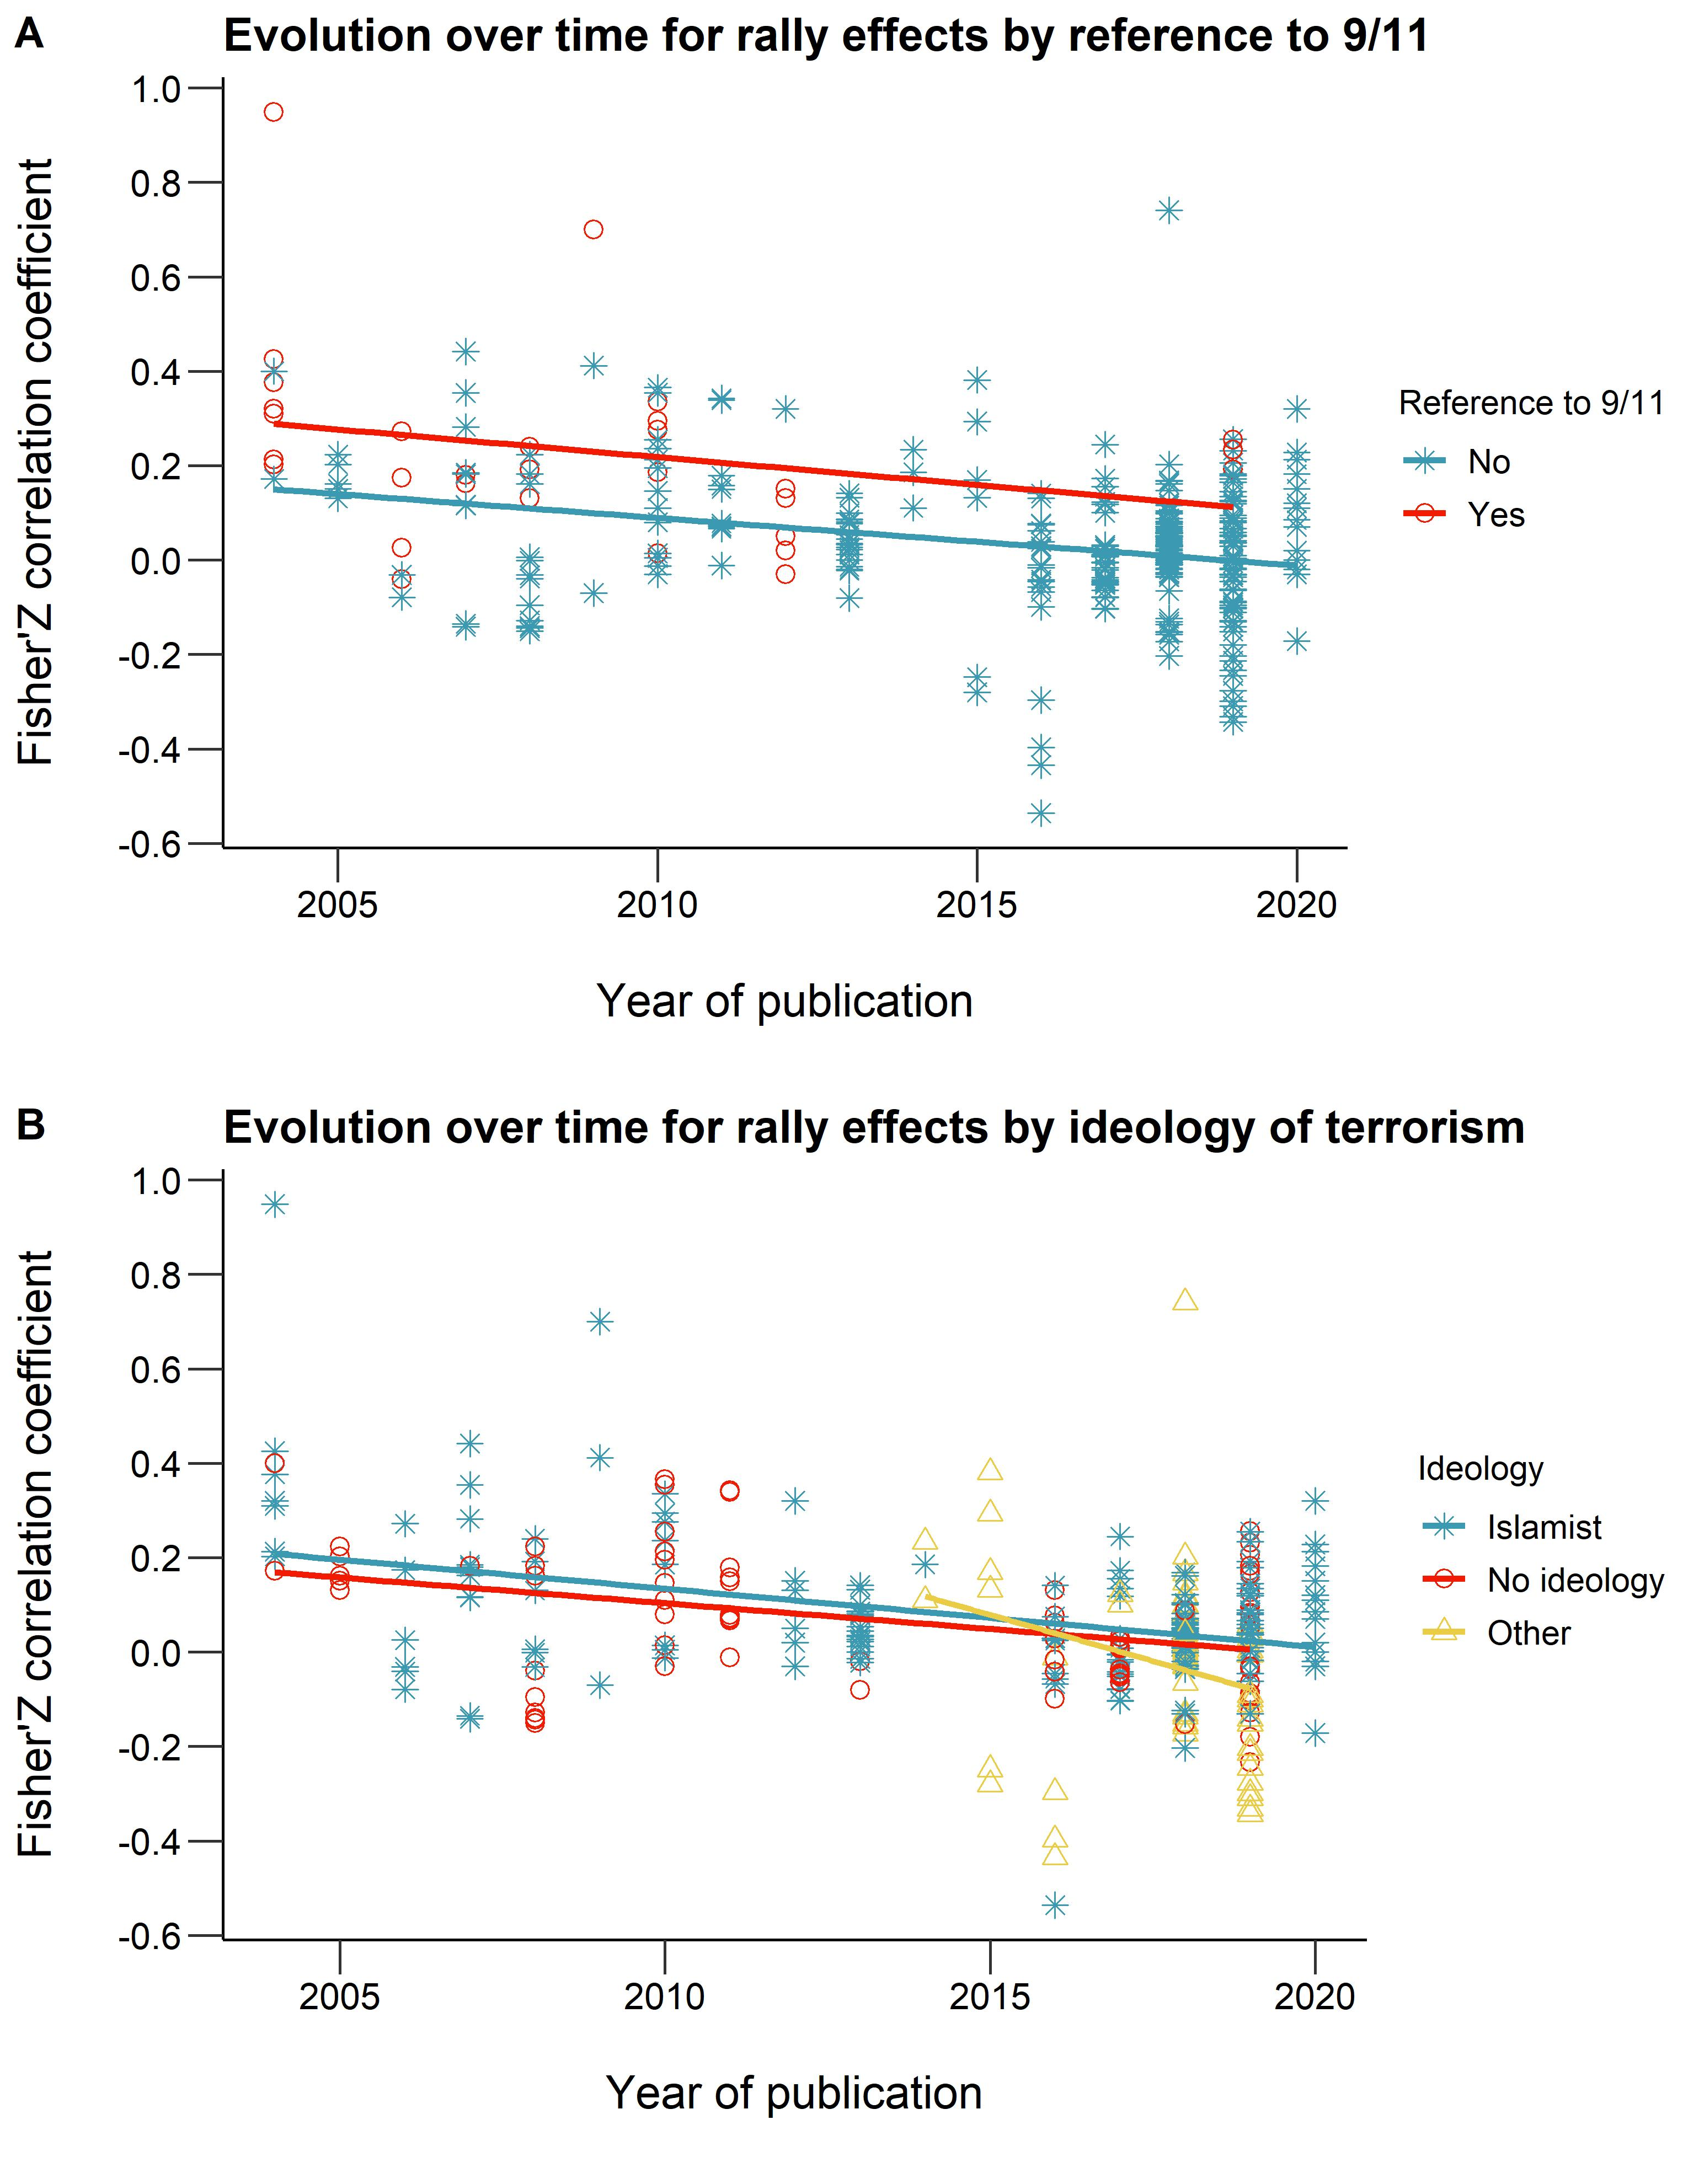
\includegraphics[width=\textwidth]{Chapter_5/art4-figure3.jpeg}
\caption[Fisher’s Z Transformed Correlation Coefficients for Rally-'Round-the-Flag Studies Regressed on Year of Publication]{\textbf{Fisher’s Z Transformed Correlation Coefficients for Rally-'Round-the-Flag Studies Regressed on Year of Publication.} \textbf{(A)} Evolution over time for studies with and without a reference to 9/11. \textbf{(B)} Evolution over time by ideology of terrorism.}
\label{fig:art4-fig3}
\end{figure}

\newpage

\begin{ThreePartTable}
\setlength{\tabcolsep}{4.5pt}
\begin{TableNotes}
\vspace{-4mm}
\footnotesize
\singlespacing
\item\textit{Note}: $k$ = number of effect sizes in the category. $b$ = unstandardized regression coefficient. The regression coefficients for the categorical variables can be interpreted as the mean effect size (i.e. Fisher’s Z correlation coefficient) for each category. Effect sizes belonging to one categorical variable that do not share subscripts differ at $p < .05$ after Benjamini-Hochberg correction for multiple comparisons. LBCI = Likelihood-Based Confidence Interval. LRT = Likelihood Ratio Test. $R^2$ refers to the proportion of the explained total variance across the levels.
\end{TableNotes}
\begin{longtable}[c]{llcrrcc}
\caption[Moderator Analyses for Rally Hypothesis]{\textbf{Moderator Analyses for Rally Hypothesis.} \\\textbf{(PANEL A)} Models as a Function of Characteristics of the Independent Variables. \\\textbf{(PANEL B)} Models as a Function of Characteristics of the Dependent Variable. \\\textbf{(PANEL C) }Models as a Function of Sample and Study Characteristics.}
\label{tab:art4-tab6}
\small \\
\toprule
\multicolumn{7}{l}{\textbf{PANEL A. CHARACTERISTICS OF THE INDEPENDENT VARIABLE}} \\
\hline
\endfirsthead
%
\multicolumn{7}{c}%
{{Table \thetable\ continued \dots}} \\
\hline
\endhead
%
\hline
\multicolumn{7}{r}{\textit{Continued on next page}} \\
\endfoot
\hline
\insertTableNotes  % tell LaTeX where to insert the contents of "TableNotes"
\endlastfoot
%
\multicolumn{2}{l}{{Moderator}} & \multicolumn{1}{c}{{$k$}} & \multicolumn{1}{c}{{$b$}} & \multicolumn{1}{c}{{95\% LBCI}} & \multicolumn{1}{c}{{$R^2$}} & \multicolumn{1}{c}{{LRT Statistic}} \\ \hline
\multicolumn{2}{l}{Ideology} & 346 &  &  & .072 & $\chi^2(2)=2.499, p=.287$ \\
 & Islamist\textsubscript{a} & 182 & .096 & [.055, .138] &  &  \\
 & Non-Islamist\textsubscript{a} & 86 & .055 & [-.004, .115] &  &  \\
 & No ideology\textsubscript{a} & 78 & .096 & [.040, .154] &  &  \\
\multicolumn{2}{l}{Measurement} & 346 &  &  & .018 & $\chi^2(4)=2.420, p=.659$ \\
 & Obj. exposure\textsubscript{a} & 108 & .105 & [.037, .175] &  &  \\
 & Subj. exposure\textsubscript{a} & 24 & .120 & [.044, .196] &  &  \\
 & Cognitions (threat)\textsubscript{a} & 119 & .093 & [.044, .144] &  &  \\
 & Emotions (anger, fear)\textsubscript{a} & 57 & .073 & [.020, .127] &  &  \\
 & Residual category\textsubscript{a} & 38 & .069 & [-.010, .149] &  &  \\
\multicolumn{2}{l}{Reference to 9/11} & 346 & .167 & [.087, .245] & .323 & $\chi^2(1)=15.190, p<.001$ \\ [1.5ex] \hline
 \multicolumn{7}{l}{\textbf{PANEL B. CHARACTERISTICS OF THE DEPENDENT VARIABLE}} \\ \hline
 \multicolumn{2}{l}{{Moderator}} & \multicolumn{1}{c}{{$k$}} & \multicolumn{1}{c}{{$b$}} & \multicolumn{1}{c}{{95\% LBCI}} & \multicolumn{1}{c}{{$R^2$}} & \multicolumn{1}{c}{{LRT Statistic}} \\ \hline
\multicolumn{2}{l}{Outcome measure} & 346 &  &  & .138 & $\chi^2(2)=5.220, p=.074$ \\
 & Politicians\textsubscript{a} & 56 & .139 & [.073, .207] &  &  \\
 & Political trust\textsubscript{a} & 177 & .046 & [-.007, .101] &  &  \\
 & Patriotism\textsubscript{a} & 113 & .101 & [.056, .145] &  &  \\
\multicolumn{2}{l}{Reference to Republican} & 346 & .062 & [.010, .115] & .078 & $\chi^2(1)=5.509, p=.019$ \\
\multicolumn{2}{l}{Reference to incumbent} & 346 & .074 & [.008, .141] & .120 & $\chi^2(1)=4.805, p=.028$ \\
\multicolumn{2}{l}{Reference to Pres. Bush} & 346 & .194 & [.101, .287] & .202 & $\chi^2(1)=16.150, p<.001$ \\ [1.5ex] \hline
 \multicolumn{7}{l}{\textbf{PANEL C. CHARACTERISTICS OF THE SAMPLE AND STUDY}} \\ \hline
 \multicolumn{2}{l}{{Moderator}} & \multicolumn{1}{c}{{$k$}} & \multicolumn{1}{c}{{$b$}} & \multicolumn{1}{c}{{95\% LBCI}} & \multicolumn{1}{c}{{$R^2$}} & \multicolumn{1}{c}{{LRT Statistic}} \\ \hline
\multicolumn{2}{l}{Research design} & 346 &  &  & .009 & $\chi^2(2)=0.616, p=.735$ \\
 & Experimental\textsubscript{a} & 81 & .100 & [.028, .175] &  &  \\
 & Correlational\textsubscript{a} & 149 & .108 & [.041, .176] &  &  \\
 & Other\textsubscript{a} & 116 & .081 & [.034, .129] &  &  \\
\multicolumn{2}{l}{Interval between IV-DV} & 346 &  &  & .015 & $\chi^2(1)=1.822, p=.177$ \\
 & Yes: interval\textsubscript{a} & 109 & .138 & [.061, .218] &  &  \\
 & No: direct\textsubscript{a} & 237 & .080 & [.040, .122] &  &  \\
\multicolumn{2}{l}{Sampling protocol} & 346 &  &  & .022 & $\chi^2(2)=1.918, p=.383$ \\
 & General population\textsubscript{a} & 172 & .071 & [.012, .132] &  &  \\
 & Student sample\textsubscript{a} & 90 & .089 & [.028, .150] &  &  \\
 & Convenience sample\textsubscript{a} & 84 & .133 & [.063, .210] &  &  \\
\multicolumn{2}{l}{Country} & 346 &  &  & .242 & $\chi^2(2)=13.565, p=.001$ \\
 & U.S.\textsubscript{a} & 101 & .159 & [.110, .211] &  &  \\
 & Israel\textsubscript{b} & 192 & .004 & [-.082, .091] &  &  \\
 & Other\textsubscript{b} & 53 & .051 & [.003, .101] &  &  \\
\multicolumn{2}{l}{Mean age} & 293 & .003 & [.000, .005] & .056 &  \\
\multicolumn{2}{l}{Percentage women} & 286 & .001 & [-.001, .003] & .007 &  \\
\multicolumn{2}{l}{Data collection year} & 322 & .004 & [-.006, .014] & .003 &  \\
\multicolumn{2}{l}{Publication year} & 346 & -.014 & [-.020, -.008] & .285 & $\chi^2(1)=16.661, p<.001$ \\* \bottomrule
\end{longtable}
\end{ThreePartTable}


\subsection{Publication Bias}
Although I attempted to minimize publication bias by means of an exhaustive search strategy, it is nevertheless important to check whether such bias is present in this meta-analysis. To this end, I used various techniques. First, I compared the effect sizes for published versus unpublished studies for each of the hypotheses. For none of the hypotheses, significant differences were found between published and unpublished studies. Furthermore, neither the effective sample size nor the inverse standard error or variance moderated the correlations between terrorism and any of the sociopolitical attitude clusters (see Table \ref{tab:art4-app-tab2} in Appendix \ref{app:E3} for all corresponding coefficients). Last, the funnel plots (Figure \ref{fig:art4-fig4}) also suggest minimal publication bias given that studies are distributed approximately symmetrical around the mean effect size. In sum, there is not much reason to be concerned about a file drawer problem. 


There is one exception, however. Figure \ref{fig:art4-fig4} also displays the summary effect based on the studies included in the meta-analysis and on studies necessary to counter publication bias (imputed by the trim and fill method). While imputing studies does not affect the results for the outgroup hostility and conservative shift hypothesis, there is some indication that it would substantially decrease the overall rally-‘round-the-flag effect (Figure \ref{fig:art4-fig4}C), which adds to the overarching conclusion that rally-effects might be idiosyncratic.


\begin{figure}[H]
\centering
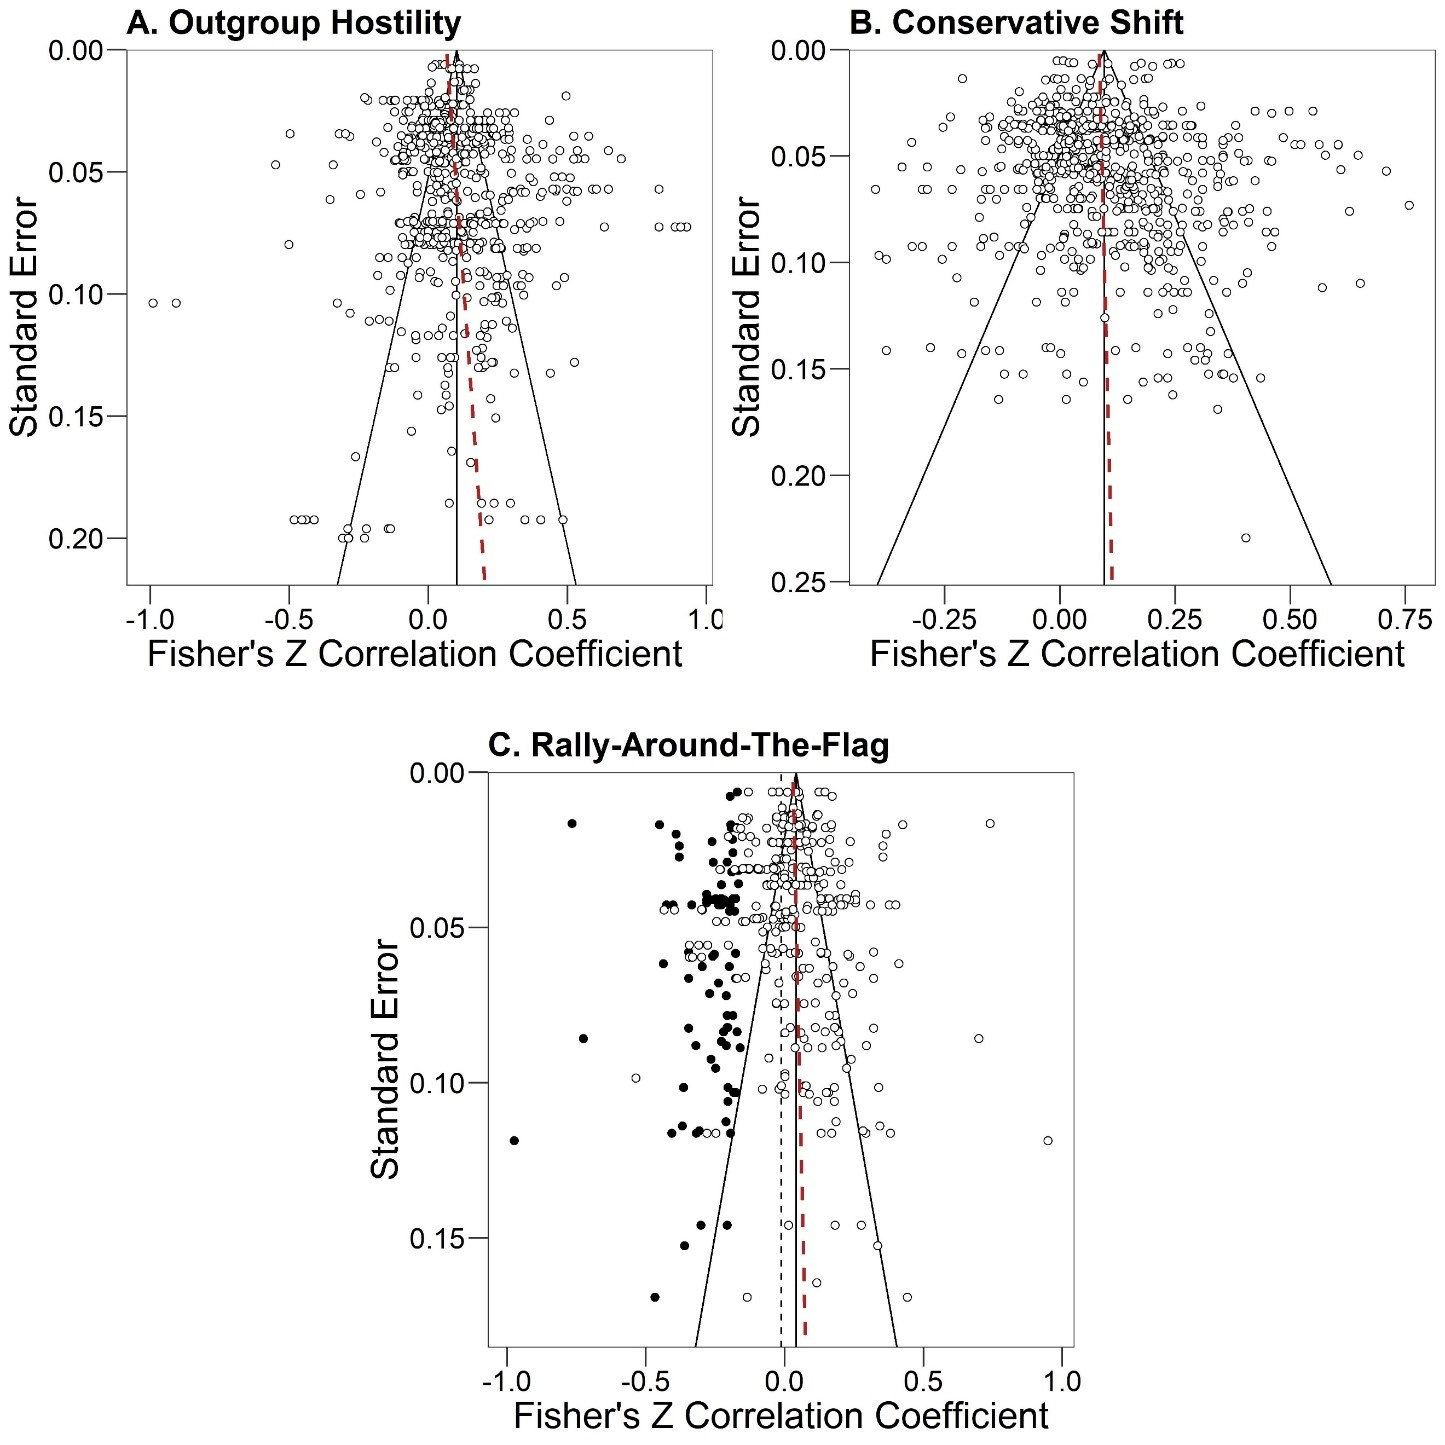
\includegraphics[width=0.98\textwidth]{Chapter_5/art4-figure4.jpg}
\caption[Funnel Plots for (A) Out-Group Hostility, (B) Conservative Shift, and (C) Rally-'Round-the-Flag Hypothesis]{\textbf{Funnel Plots for (A) Out-Group Hostility, (B) Conservative Shift, and (C) Rally-'Round-the-Flag Hypothesis.}  Scatter plot displaying the standard errors on a reversed axis against the observed (open circles) and trim-and-fill imputed (filled circles) effect sizes. Summary effect in solid black lines, summary effect including imputed studies in dotted black lines, and Egger’s regression line in dotted red lines.}
\label{fig:art4-fig4}
\end{figure}
\newpage


\section{Conclusion}
Scholars, policymakers, and the public alike often assume that terrorism is effective to the extent it is able to affect the electorate \citep{Crenshaw1986}. But, does terrorism really affect citizens' political attitudes? If so, how and to what extent? On the one hand, this meta-analysis confirms that terrorism exposure—be it in terms of self-reported exposure, manipulated news exposure, exposure to a naturally occurring attack, anxious or angry appraisals of terrorism, or terrorist risk perceptions—is related to higher levels of out-group hostility, political conservatism, and, albeit to a weaker extent, rally-‘round-the-flag responses. On the other hand, important features of this field of study warrant a certain caution in drawing general conclusions. Indeed, at its core, this review revealed that the study of public responses to terrorism is in practice limited to a much narrower question: Does \textit{Islamist} terrorism affect attitudes within \textit{Western} societies?

First, the vast majority of studies in this body of scholarship examine threats or a handful of particular acts of Islamist terrorism (or refrain from identifying a specific ideology). This is unfortunate because comparing across cases of terrorism with different ideological motives would allow scholars to separate those responses that are unique to Islamist terrorism (in Western contexts, \textit{infra}) from more general political-psychological coping mechanisms. In this respect, the empirical evidence indicates that Islamist terrorism is related to out-group hostility and in-group solidarity, whereas attitudinal responses to violence perpetrated by non-Islamist actors look quite different. Here, the overall effect sizes are much weaker (for conservative-shift outcomes) or non-significant (for out-group hostility and rallying outcomes). This suggests that it might not be the threat of violence per se that is driving public reactions to terrorism, as is often assumed, but rather the threat of violence perpetrated by specific, often out-group, actors. However, this is a hypothesis calling for further scrutiny, as currently only a handful of studies look beyond Islamist (or unspecified) terrorism.

Given the recent upsurge in far-right terrorism \citep{TheInstituteForEconomicsAndPeace2019}, it seems particularly pertinent to understand how citizens react to this type of violence and how these responses meaningfully differ from responses to other types of violence. Certainly, as others have noted before \citep{Meier2020b}, unpacking the causes and consequences of far-right violence has received extensive attention in the literature \citep[e.g.,][]{Caiani2012, Koopmans2004, Simpson2018}, yet these acts of political violence are rarely described as ‘terrorism’ within scholarly work. This review shows how this semantic choice inhibits the exchange of knowledge between work on far-right violence and work on other types of political violence more regularly called ‘terrorism’ (such as Islamist violence), thereby reducing opportunities to detect whether theories and findings travel across ideological lines.

Second, much of the literature is still focused on the United States, and particularly the political aftermath of 9/11, or on the Israeli-Palestinian conflict. Again, while this has provided valuable insights, generalizations beyond these specific contexts may be, at best, complicated. Rally-‘round-the-flag mechanisms, for example, seem to be primarily driven by a rally-‘round President Bush effect in the wake of 9/11, and terrorism-induced reactions of out-group hostility or political conservatism are also substantially weaker outside an American or Israeli context. More generally, many of our extant expectations ignore particularities of the countries studied and their historical, institutional and cultural differences with other countries. Specifically, studies conducted in regions that have a history of being vulnerable to terrorist violence (e.g., Afghanistan, Iraq, Syria, Nigeria, and Pakistan) are missing in the current literature. As a result, we still know surprisingly little about how people in countries most affected by terrorism cope with such severe and sustained threat. Yet, the focus on the United States and Israel might not be entirely caused by the field being dominated by scholars studying these countries. It might also be that studies conducted in these non-Western countries are more often published in different languages and outlets (and, hence, were not retrieved) or use different terms to denote the violence (and, hence again, were not retrieved).

Last, the review exposed some additional methodological gaps and issues which, in turn, give rise to other promising directions for future research. For example, a large majority of studies still tend to be under-powered and drawn from convenience samples, and only a handful of studies were preregistered before data collection. Also, the meta-analysis seems to support the notion that public reactions to terrorism are fairly short-lived—at least for out-group hostility studies. Yet, the dearth of longitudinal research on the impact of terrorism on attitudes makes it hard to draw firm conclusions in this respect. In sum, to gain a deeper and more nuanced understanding of how terrorism is changing citizens, more research is warranted. Especially, more preregistered, adequately powered, representative, longitudinal, and non-Western research focused on violence perpetrated by a wider range of actors would allow scholars to disentangle who reacts to which type of terrorism, how, and for how long. Only such nuanced understanding of public reactions to terrorism can bring about effective remedies to potential democratic backlashes in times of terror.


\begin{comment}
\subsubsection{Who Is Being Studied?}
Studies on the relationship between terrorism and attitudes are conducted among the general population (115 studies, 37\%), student samples (107 studies, 34\%), and other convenience samples (such as online opt-in panels, snowball samples, or online/social media samples; 92 studies, 29\%). The mean age across all samples is 33.11 years (SD = 11.43) and studies include 55\% women on average (SD = 14.24). Most studies examine the opinions of a majority group in the country of study (e.g., whites in the US, Israeli Jews in Israel; 136 studies, 43\%) or use a mixed sample (60 studies, 19\%). Only 14 studies (4\%) are conducted among participants of minority groups. The other 104 studies do not disclose information on the ethnic composition of their sample (33\%).



\subsubsection{When and Where Do Studies Take Place?}
When and where were these respondents questioned? As Figure \ref{fig:art4-fig2} shows, academic interest in the association between terrorism and public opinion clearly commenced after the 9/11 attacks and was given an extra boost with the 2015-2016 ISIS attacks.\footnote{While 9/11 might have initiated research this topic, it is equally possible that similar research was previously not framed as “terrorism” research.} 

\begin{figure}[H]
\centering
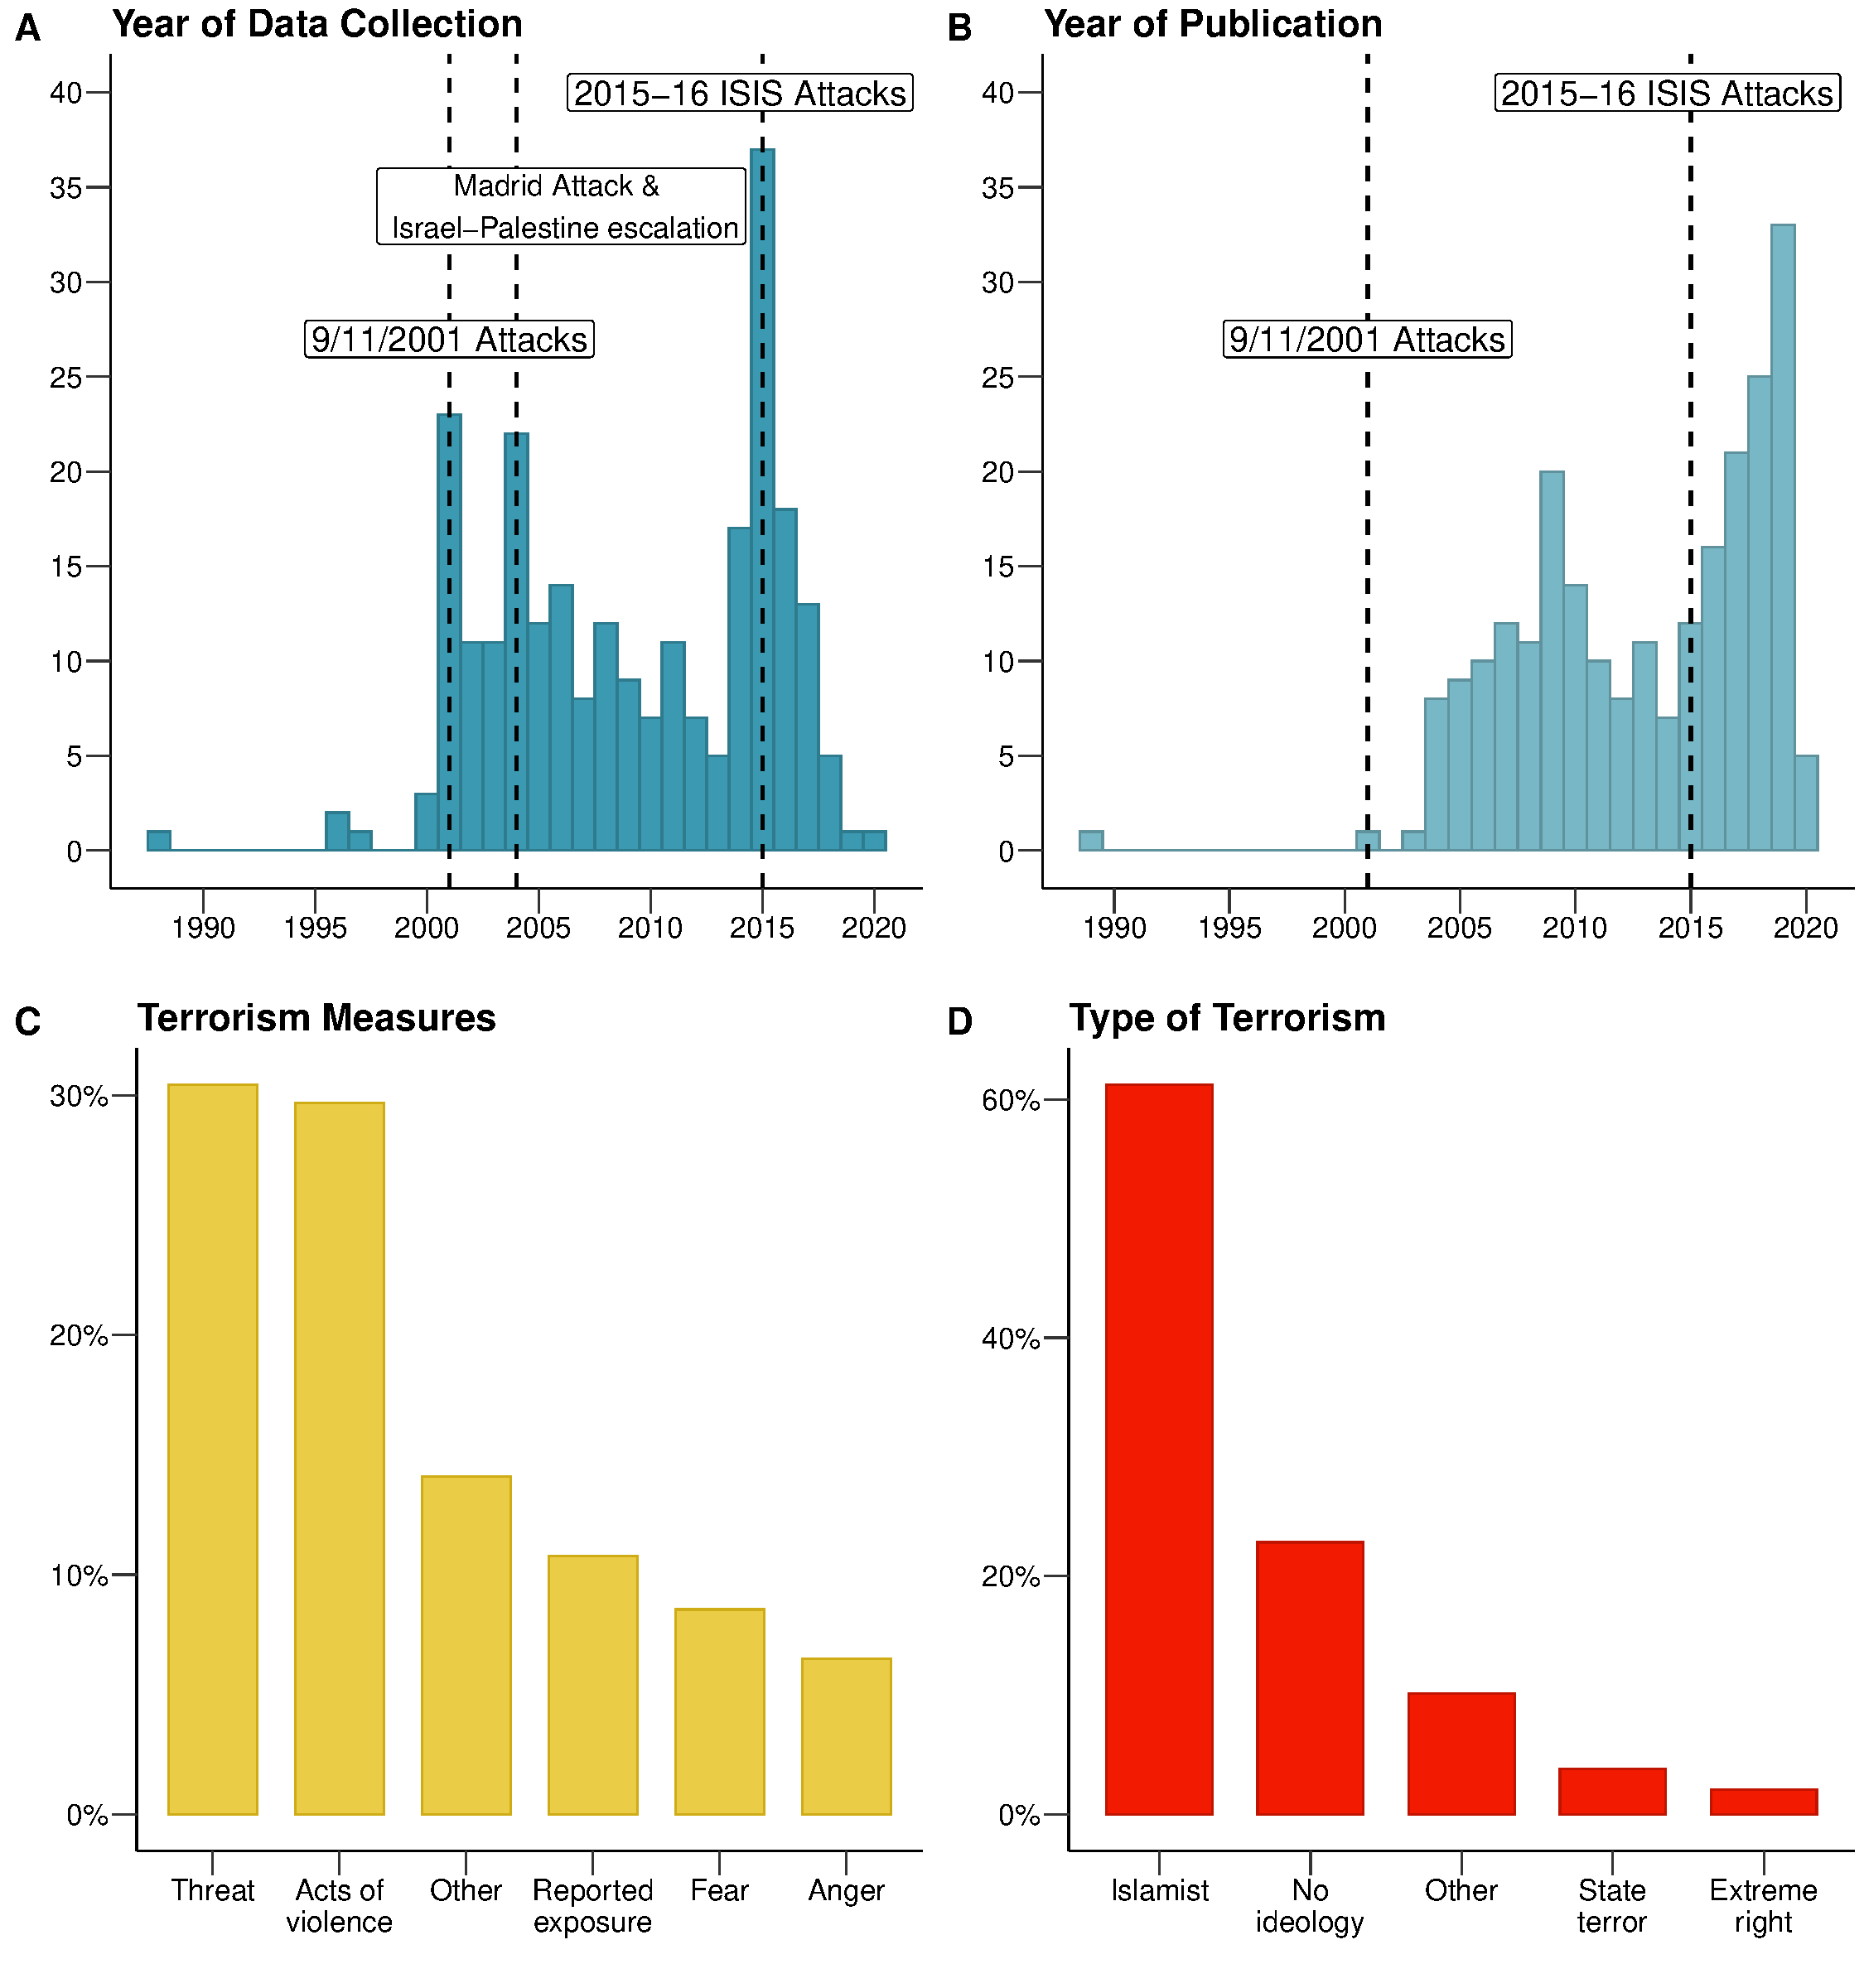
\includegraphics[width=\textwidth]{Chapter_5/art4-figure2.pdf}
\caption{Number of Studies per Year of Data Collection and Publication}
\label{fig:art4-fig2}
\end{figure}


Furthermore, the geographical scope of this field of study is limited. Most studies are---perhaps unsurprisingly---conducted in the United States (116 studies, 37\%) and Israel (62 studies, 20\%). The remaining 43\% of the studies are more or less evenly distributed across 29 countries (plus the European Union). Only seven studies (2\%) are conducted in non-Western contexts (i.e., two in Nigeria and one in Egypt, Morocco, South-Africa, Colombia, and Pakistan).\footnote{Again, it is possible that the field of study focused on non-Western contexts uses a different vocabulary and were not framed as `terrorism' studies.}

\subsubsection{How Do the Research Designs Look Like?}
Besides a limited geographical scope, the review reveals some important methodological gaps related to the research designs used. Panel studies, for instance, are extremely rare in this field of study, making it hard to assess the long-term impact of terrorism. Indeed, almost half of the studies uses a cross-sectional design (47\%), with experiments and quasi-experiments used in 103 (33\%) and 41 (13\%) studies. Second, the mean statistical power across all studies included in this meta-analysis is $.53$ (SD = 0.38), which is way below the generally accepted rule of $\geq .80$. Hence, studies included in this body of scholarship tend to be underpowered, which increases the risk of both false negatives and false positives. Part of the explanation might be the fact that only ten studies (3\%) are reported as preregistered and, hence, conducted an a priori sample size calculation. In this respect, the median effective sample size is 305.5, with a minimum of 22 and a maximum of 37,670 participants (M = 1349.29, SD = 4234.44). 


\subsubsection{What Are Commonly Used Treatments and Measures of Terrorism?}
Exposure to terrorism is measured in various ways. Sometimes participants were exposed to a news article or video clip about a particular act of violence, whereas at other times exposure happened more naturally when a terror attack occurred at the same time a survey was being fielded. Sometimes studies gauged or manipulated citizens’ perception of the threat of terrorism, while other studies were more interested in affective appraisals. And yet other studies asked respondents to report their own and relatives’ exposure to specific acts of violence. Table \ref{tab:art4-tab2} contains the most common ways used in the literature to grasp terrorism exposure, whereas Figure 5.3 (panel A) on the next page displays the relative distribution of the main categories.

%---------------------------------------
% TABLE 2
%---------------------------------------
\vspace{3mm}
\begin{longtable}{@{}lp{10cm}@{}}
\caption{Measures and Manipulations Used to Gauge Citizens’ Exposure to or Appraisals of Terrorism}
\small \\
\toprule
Main category & Specific measures \\* \midrule
\endfirsthead
%
\multicolumn{2}{c}%
{{Table \thetable\ continued \dots}} \\
\toprule
Main category & Specific measures \\* \midrule
\endhead
\hline
\multicolumn{2}{r}{\textit{Continued on next page}} \\
\endfoot
\hline
\endlastfoot
%
Objective exposure & Pre- and post-violence \\
 & Days in-between act of violence and survey day \\
 & Newspaper vignette of act of violence \\
 & News clip of act of violence \\
 & Terrorism (vs. crime) wording of the questions \\
Self-reported exposure & Direct exposure to terrorism (e.g., witnessed, being   injured) \\
 & Indirect exposure via friends and family \\
 & Media exposure \\
Cognitions & Self-reported concern/worry to become a victim of terrorism \\
 & Self-reported concern/worry for an attack on the nation \\
 & Manipulated vignette or writing task on the personal/national threat of terrorism \\
 & Manipulated percentage of the threat of terrorism \\
 & Remuneration of the threat of terrorism for oneself \\
Emotions & Anger/outrage (targeted at the phenomenon terrorism as such or at a particular attack or terrorist organization) \\
 & Fear/anxiety (idem) \\
 & Sadness (idem) \\
 & General negative valence (idem) \\
Other & Depression caused by terrorism \\
 & Post-Traumatic Stress Disorder caused by terrorism \\
 & Loss of resources (e.g., economic losses) \\* \bottomrule
\end{longtable}

%---------------------------------------
% FIGURE 3
%---------------------------------------
\begin{figure}[H]
\centering
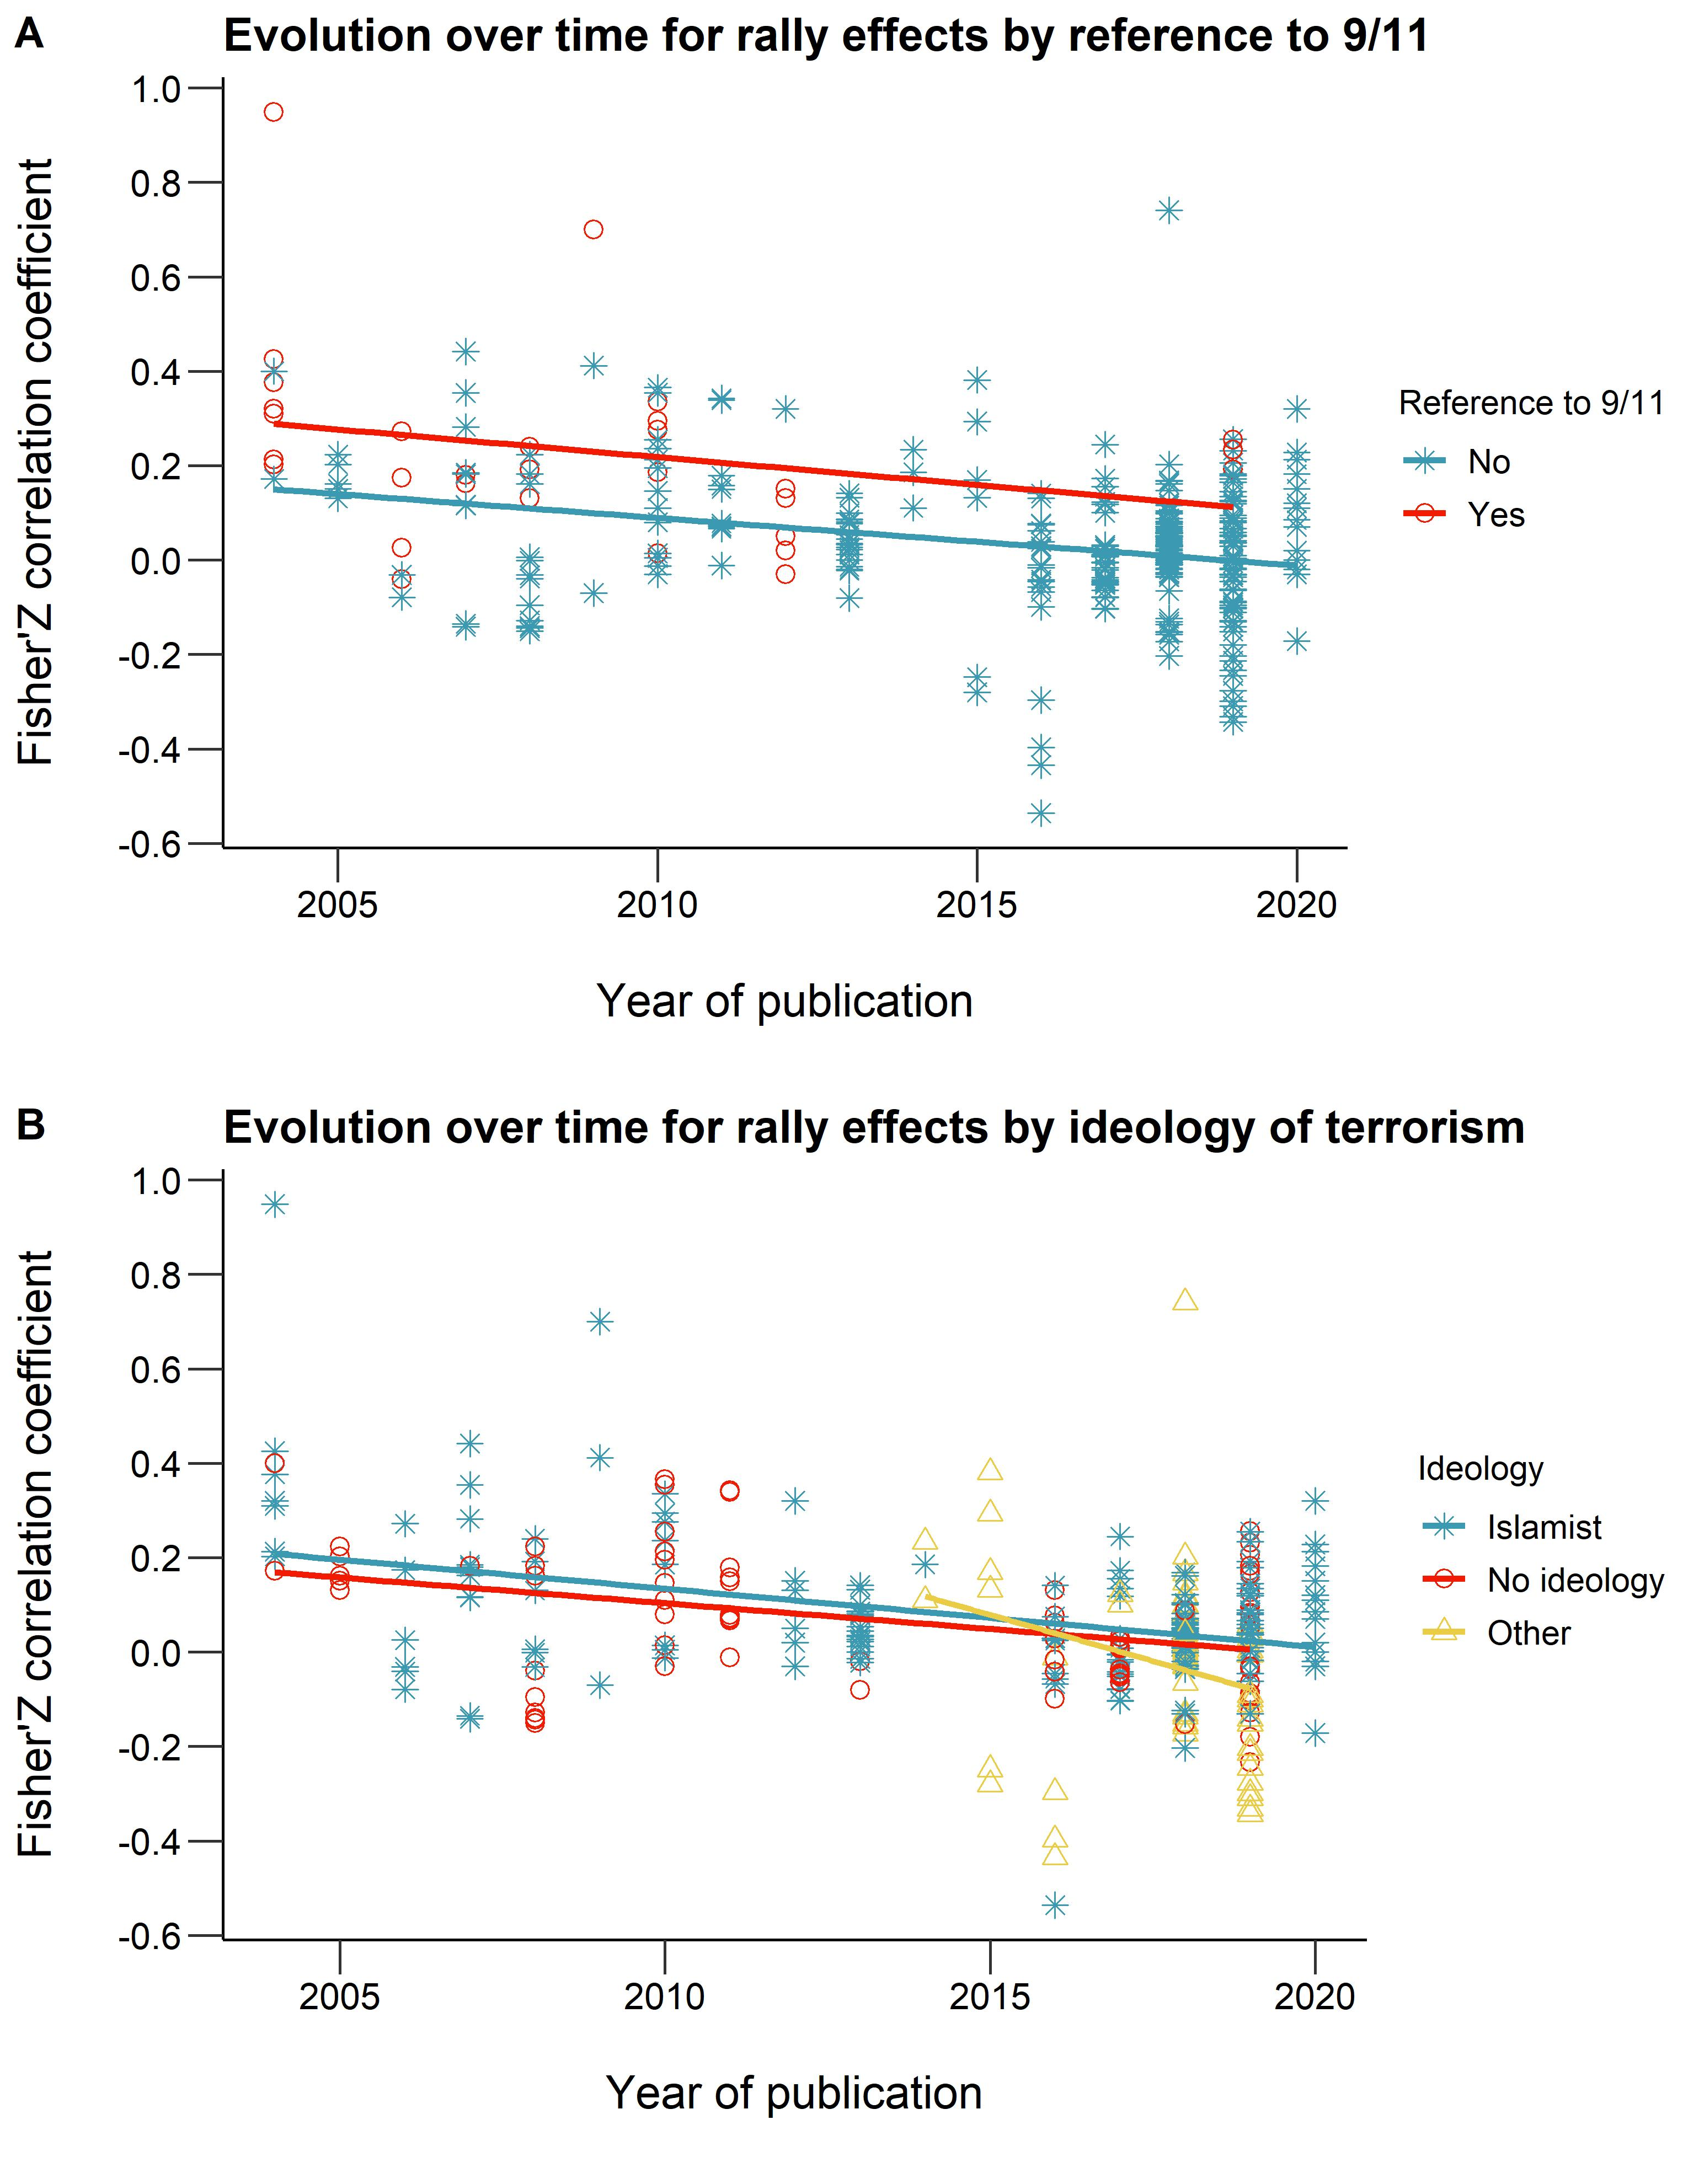
\includegraphics[width=\textwidth]{Chapter_5/art4-figure3.pdf}
\caption{Distribution of Terrorism Measures/Manipulations and Types/Ideology}
\label{fig:art4-fig3}
\end{figure}
%---------------------------------------

As Figure \ref{fig:art4-fig3}A shows, most effect sizes describe the impact of cognitive threat perceptions (30\%) or `objective' exposure measured via a (quasi-)experimental designs (29\%). The most frequently studied acts of violence are 9/11, the Israeli-Palestinian conflict, and the Paris attacks. Consequently, regarding the type/ideology of terrorism (Fig. 5.3B), the vast majority of studies refers to Islamist terrorism (974 data points, 58\%), whereas the share of studies on how the pubic reacts to extreme-right terror is remarkably low (39 data points, 2\%). It is interesting to note in this respect that only a handful of studies includes an explicit definition of `terrorism'---leading to the implicit assumption that ‘terrorism’ is a clear-cut ‘you-know-it-when-you-see-it’ phenomenon.
%\footnote{This puts the field of empirical terrorism studies in sharp contrast with the field of critical terrorism studies which engages extensively with the definition of terrorism. The lack of exchange between both fields is quite remarkable.}


\subsubsection{What Are Commonly Used Measures of Sociopolitical Attitudes?}

Last, as mentioned before, this body of scholarship tends to focus on three clusters of outcome measures. That is, studies include measures pertaining to (1) out-group hostility, including cognitive (e.g., stereotypes, prejudices, distrust), affective (e.g., feeling thermometers, xenophobia/fear, hatred), behavioral (e.g., helping, harming, social distance, avoidance), or policy-related (e.g., support for anti-immigration policies) attitudes; (2) a conservative shift, including support for specific policies (e.g., military intervention, enhanced national security)\footnote{Anti-out-group policy attitudes are studied under the out-group hostility cluster (and not under the conservative shift cluster). First, these outcome variables include qualitatively different information on, for example, the target out-group of interest. Second, although one could argue that anti-out-group policy attitudes empirically correlate with conservatism, it is questionable whether they conceptually represent the same underlying construct (i.e., conservatism). } and general political beliefs (e.g., RWA, SDO, political self-placement), and (3) rally effects, including support for national leaders (e.g., presidential approval) and general attachment to the nation (e.g., patriotism, political trust). Figure \ref{fig:art4-fig4} shows the relative distribution of the outcome measures used.


\begin{figure}[H]
\centering
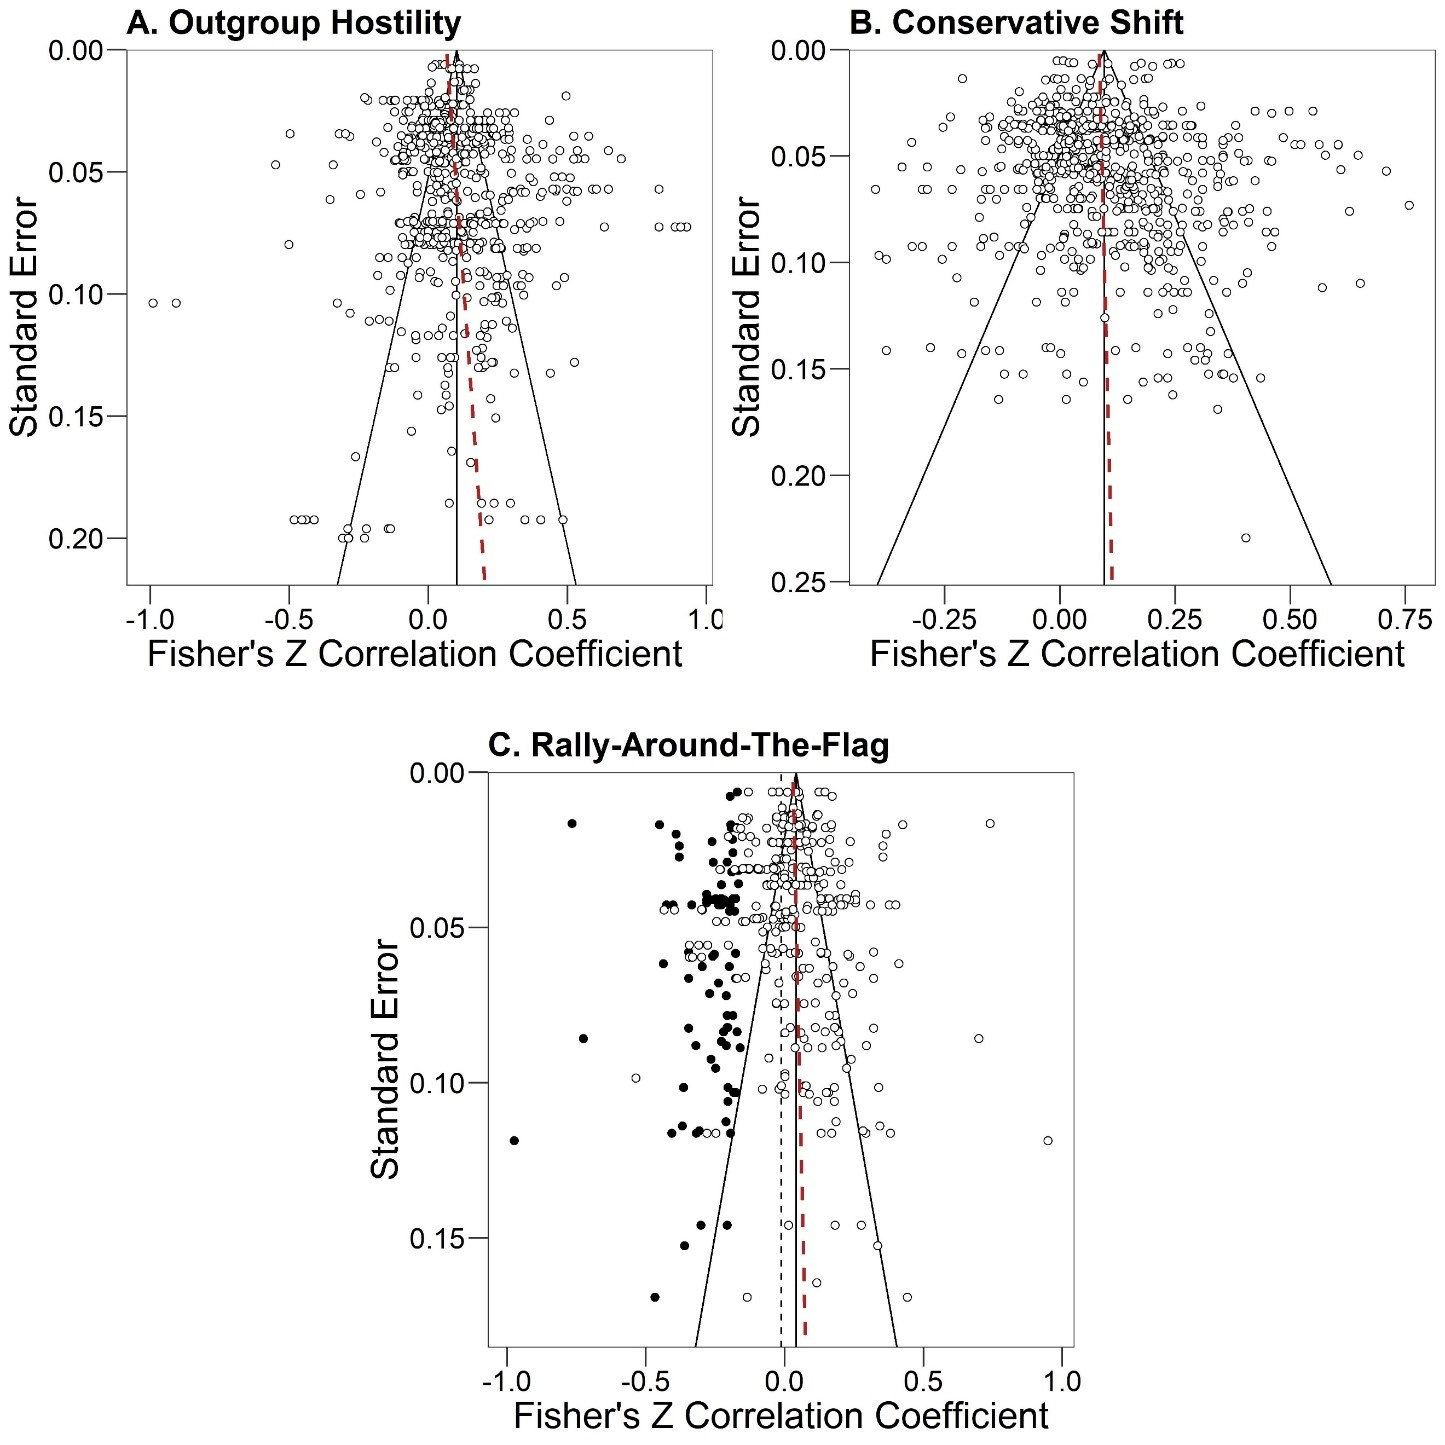
\includegraphics[width=\textwidth]{Chapter_5/art4-figure4.pdf}
\caption{Distribution of Attitudinal Outcome Measures}
\end{figure}
In what follows, a three-level meta-analysis is performed to consolidate the overall effect size for out-group hostility, conservative shift, and rally-‘round-the-flag measures. As these measures convey qualitatively different information, and might thus be affected in a different way by the studied moderators, they cannot easily be aligned with each other. Therefore, I conduct three separate meta-analyses for each type of attitudinal measure. The meta-analysis contains 678 data points (from 129 reports) testing the out-group hostility hypothesis, 688 data points (from 134 reports) testing the conservative shift hypothesis, and 319 data points (from 67 reports) on the rally-‘round-the-flag hypothesis.


\subsection{Overall Effect Size and Effect Size Heterogeneity}
To what extent is terrorism related to out-group hostility, political conservatism, or rally-‘round-the-flag responses? To answer this question, I first estimate the overall Fisher’s Z correlation coefficient based on an intercept-only three-level model. The overall estimated correlations ($Z_r$), Likelihood-Based Confidence Intervals (LCBIs), number of correlations included (\textit{k}), and heterogeneity indices for all three hypotheses are listed in Table \ref{tab:art4-tab3}. Note that all correlations are Fisher’s Z transformed. For ease of interpretation, however, the correlations mentioned in the text are backward transformed to their normal correlation scale (denoted as $\hat{\rho}$). 


Results show that terrorism is significantly associated with out-group hostility ($\hat{\rho} = .119$), political conservatism ($\hat{\rho} = .129$), and, to a lesser extent, rally-‘round-the-flag effects ($\hat{\rho} = .060$). In other words, the more someone is exposed to, concerned about, and/or angry because of terrorism, the more he/she will derogate `others,' find solace in conservative ideas, and bolster attachment to the nation and its leaders. At the same time, the effect size for such rally effects is only half that of the other two hypotheses, and all associations are small \citep{Cohen1988}.


\begin{table}[H]
\caption{Estimated Overall Fisher’s Z Effect Size Correlations, Confidence Intervals, and Heterogeneity Indices for All Three Hypotheses}
\label{tab:art4-tab3}
\begin{tabular}{@{}p{3cm}C{0.9cm}C{0.9cm}C{2.2cm}C{1cm}C{1cm}C{1cm}C{1cm}@{}}
\toprule
& $k$ & $Z_r$ & LBCI & $\tau_{(2)}^2$ & $\tau_{(3)}^2$ & $I_{(2)}^2$& $I_{(3)}^2$\\ \midrule
out-group Hostility & 678    & $.120$    & [$.088$; $.152$]  & $.009$ & $.028$ & $.242$ & $.729$\\
Conservative Shift & 688    & $.130$    & [$.105$; $.156$]  & $.012$ & $.017$ & $.395$ & $.568$\\
Rally Effects      & 319    & $.060$    & [$.025$; $.096$] & $.011 $ & $.015$ & $.422$ & $.558$\\ \bottomrule
\end{tabular}
\end{table}


Next, the heterogeneity variance estimates from the empty models (also Table \ref{tab:art4-tab3}) point to substantial differences in observed effect sizes both within and between studies for all three clusters of outcome measures. Likelihood ratio tests confirm that significant variance is present both at the between-study and within-study level for the out-group hostility ($\chi_{(3)}^2(1) = 372.067, p < .001$ and $\chi_{(2)}^2(1) = 1813.218, p < .001$), conservative shift ($\chi_{(3)}^2(1) = 208.081, p < .001$ and $\chi_{(2)}^2(1) = 2908.001, p < .001$), and rally effects ($\chi_{(3)}^2(1) = 86.639, p < .001$ and $\chi_{(2)}^2(1) = 4782.907, p < .001$) measures. This means that there are true differences between studies and between the effect sizes within a study. Therefore, a three-level model is statistically more appropriate than both a two-level random effects and a fixed effect model. In the next series of meta-regression models, I explore to what extent differences in effect sizes are moderated by additional variables.


In what follows, I provide a short description of the significant moderators for each of the hypotheses, whereas all coefficients of the separate models for each of the moderators are displayed in Table \ref{tab:art4-tab4} for the out-group hostility hypothesis, Table \ref{tab:art4-tab5} for the conservative shift hypothesis, and Table \ref{tab:art4-tab6} for the rally-‘round-the-flag hypothesis. Here, coefficients for categorical variables denote the overall effect size per category, while coefficients for continuous moderators are mean-centered unstandardized coefficients.


\subsubsection{Moderators of the Out-Group Hostility Hypothesis} 
The effect size quantifying the relationship between terrorism and out-group hostility is significantly moderated by the sampling protocol, mean age of the sample, study location, study design, and several features of the operationalization of both the independent and dependent variable. 

\vspace{3mm}
\noindent\textbf{\textit{Sample and Study Characteristics.}} While results indicate a significant positive association between terrorism and out-group hostility for different types of samples, pairwise comparisons (always with Holm-Bonferroni correction for multiple testing) indicate that the relationship between terrorism and out-group hostility is significantly weaker when using student samples compared to using general population or other convenience samples. Second, in a similar vein, the mean age in the sample positively moderated the effect size, in the sense that more positive correlations were found in older samples. Third, while results indicate a significant positive association between terrorism and out-group hostility regardless of the specific location of study, pairwise comparisons indicate that, compared to studies conducted in the United States, the relationship between terrorism and out-group hostility is significantly stronger in Israel and significantly weaker in all other countries. Furthermore, the results indicate that the effect size for correlational studies is more than twice that of studies conducting experiments. In general, the research design used turns out to be one of the strongest moderators explaining 19\% of the variance in effect sizes. In this respect, studies with a delay in-between the assessment of the independent and the dependent variable also display a significantly lower and even non-significant effect size.

\vspace{3mm}
\noindent\textbf{\textit{Characteristics of the Independent Variable.}} First and foremost, the overall effect size for those few studies examining \textit{non}-Islamist terrorism fails to reach statistical significance, whereas those studies not referring to any ideology result in the highest overall effect size. Second, the exact measurement or manipulation used to gauge terrorism also significantly explains the strength of the effect size. More specifically, pairwise comparisons indicate that objective exposure to acts of violence (measured via experiments or quasi-experiments) leads to significantly lower effect sizes compared to any other way of measuring the independent variable. Even more, the average effect size for this category fails to reach significance. Conversely, the relationship between anger appraisals and out-group hostility results in a stronger effect size, but here the comparisons fail to reach significance after Holm-Bonferroni correction due to the small number of effect sizes using anger appraisals as independent variable. 


\vspace{3mm}
\noindent\textbf{\textit{Characteristics of the Dependent Variable.}} The target out-group under scrutiny also shows a significant and strong main effect. Although terrorism is associated with significant increases in hostility towards all out-groups studied, the relationship is significantly stronger for religious out-groups and for immigrants/refugees. In addition, I also found partial support for a so-called `guilt-by-association.' More specifically, studies referring to Islamist terrorism and questioning Muslim attitudes (i.e., hard association) result in significantly stronger effect sizes compared to both studies without such association as well as to studies referring to Islamist terrorism and questioning attitudes towards immigrants and/or refugees (i.e., soft association).

	
\newpage
\begin{ThreePartTable}
\setlength{\tabcolsep}{4.5pt}
\begin{TableNotes}
\vspace{-4mm}
\footnotesize
\singlespacing
\item\textit{Note}: $k$ = number of effect sizes in the category. $b$ = regression coefficient. The regression coefficients for the categorical variables can be interpreted as the mean effect size for each category. Effect sizes belonging to one categorical variable that do not share subscripts differ at $p<.05$ after Holm-Bonferroni correction for multiple comparisons. LBCI = Likelihood-Based Confidence Interval. LRT = Likelihood Ratio Test. $R^2$ refers to the proportion of the explained total variance across the levels.
\end{TableNotes}
\begin{longtable}[c]{llcrrcc}
\caption[Meta-Regression Models for Out-Group Hostility Hypothesis]{\textbf{Meta-Regression Models With One Moderator for Out-Group Hostility Hypothesis.} \textbf{(PANEL A)} Models as a Function of Sample and Study Characteristics. \textbf{(PANEL B)} Models as a Function of Characteristics of the Independent Variables. \textbf{(PANEL C)} Models as a Function of Characteristics of the Dependent Variable. }
\small \\
\toprule
\multicolumn{7}{l}{\textbf{PANEL A. SAMPLE AND STUDY CHARACTERISTICS}} \\
\hline
\endfirsthead
%
\multicolumn{7}{c}%
{{Table \thetable\ continued \dots}} \\
\hline
\endhead
%
\hline
\multicolumn{7}{r}{\textit{Continued on next page}} \\
\endfoot
\hline
\insertTableNotes  % tell LaTeX where to insert the contents of "TableNotes"
\endlastfoot
%
\multicolumn{2}{l}{{Moderator}} & \multicolumn{1}{c}{{$k$}} & \multicolumn{1}{c}{{$b$}} & \multicolumn{1}{c}{{95\% LBCI}} & \multicolumn{1}{c}{{$R^2$}} & \multicolumn{1}{c}{{LRT Statistic}} \\ \hline
\multicolumn{2}{l}{Sampling protocol} & 678 & & & $.078$ &  $\chi^2(2)=22.482, p<.001$  \\
  & General population\textsubscript{a}  & 221 & $.148$ & [$.101, .195$] & & \\
  & Student sample\textsubscript{b}      & 247 & $.053$  & [$.009, .097$] & & \\
  & Convenience sample\textsubscript{c}  & 210 & $.169$ & [$.121, .218$] & & \\
 \multicolumn{2}{l}{Mean age}  & 521 & $.004$ & [$.002, .006$] & $.089$ & \\
 \multicolumn{2}{l}{Percentage women} & 620 & $.002$ & [$-.001, .003$] & $.029$ &\\
 \multicolumn{2}{l}{Publication year} & 678 & $-.003$ & [$-.010, .003$] & $.010$ & $\chi^2(1)=1.200, p=.273$  \\
  \multicolumn{2}{l}{Data collection year} & 542 & $-.003$ & [$-.009, .002$] & $.013$ &  \\
 \multicolumn{2}{l}{Country} & 678 &  &  & $.063$ &  $\chi^2(1)=6.343, p=.042$   \\
  & US\textsubscript{a}     & 188  & $.135$ & [$.085, .185$] &  &  \\
  & Israel\textsubscript{a} & 176  & $.180$ & [$.111, .249$] &  &  \\
  & Other\textsubscript{b}  & 314  & $.080$ & [$.035, .125$] &  &  \\
\multicolumn{2}{l}{Research Design} & 263 &  &  & $.191$ & $\chi^2(2)=22.850, p<.001$  \\
 & Experimental\textsubscript{a}  & 167 & $.088$ & [$.036, .141$] &  &   \\
 & Correlational\textsubscript{b}  & 297 & $.181$ & [$.143, .220$] & & \\
 & Other\textsubscript{c}          & 214 & $.124$ & [$.055, .193$] &  & \\
  \multicolumn{2}{l}{Time interval} & 678 & $-.085$ & [$-.142, -.028$] & $.058$ & $\chi^2(1)=8.403, p=.004$  \\[1.5ex] \hline
 \multicolumn{7}{l}{\textbf{PANEL B. CHARACTERISTICS OF THE INDEPENDENT VARIABLE}} \\ \hline
 \multicolumn{2}{l}{{Moderator}} & \multicolumn{1}{c}{{$k$}} & \multicolumn{1}{c}{{$b$}} & \multicolumn{1}{c}{{95\% LBCI}} & \multicolumn{1}{c}{{$R^2$}} & \multicolumn{1}{c}{{LRT Statistic}} \\ \hline
\multicolumn{2}{l}{Ideology}    & 678 & & & $.054$ & $\chi^2(2)=11.496, p=.003$  \\
 & Islamist\textsubscript{a}     & 459 & $.111$ & [$.076, .146$] &  &   \\
 & Non-Islamist\textsubscript{a,b} & 68 & $.050$ & [$-.016, .115$] &  & \\
 & No ideology\textsubscript{b}  & 151 & $.180$ & [$.130, .228$] & & \\ 
\multicolumn{2}{l}{Reference to 9/11} & 678 & $-.057$ & [$-.145, .032$] & $.016$ & $\chi^2(1)=1.581, p=.209$  \\
\multicolumn{2}{l}{Measurement}  & 678 & & & $.159$ & $\chi^2(5)=34.741, p<.001$  \\
 & Acts of violence\textsubscript{a}    & 249 & $.043$ & [$-.004, .090$] &  &   \\
 & Self-r. exposure\textsubscript{a,b} & 67  & $.109$ & [$.060, .158$] &  & \\
 & Threat perception\textsubscript{b}   & 187 & $.190$ & [$.149, .232$] & & \\
 & Fear\textsubscript{b}              & 44  & $.141$ & [$.088, .195$] &  & \\
 & Anger\textsubscript{b}               & 29  & $.213$ & [$.153, .273$] & & \\
 & Other\textsubscript{b}               & 102 & $.128$ & [$.080, .177$] & & \\ [1.5ex] \hline
 \multicolumn{7}{l}{\textbf{PANEL C. CHARACTERISTICS OF THE DEPENDENT VARIABLE}} \\ \hline
 \multicolumn{2}{l}{{Moderator}} & \multicolumn{1}{c}{{$k$}} & \multicolumn{1}{c}{{$b$}} & \multicolumn{1}{c}{{95\% LBCI}} & \multicolumn{1}{c}{{$R^2$}} & \multicolumn{1}{c}{{LRT Statistic}} \\ \hline
\multicolumn{2}{l}{Measurement}  & 678 & & & $.036$ & $\chi^2(3)=12.137, p=.007$  \\
 & Affective\textsubscript{a}    & 197 & $.146$ & [$.108, .185$] &  & \\
 & Cognitive\textsubscript{a,b}    & 262 & $.117$ & [$.081,  .153$] & & \\
 & Behavioral\textsubscript{b}   & 46  & $.054$ & [$-.002, .110$] & & \\
 & Political\textsubscript{a,b}    & 173 & $.120$ & [$.079,  .161$] & & \\
\multicolumn{2}{l}{Target out-group}  & 678 & & & $.044$ & $\chi^2(2)=14.287, p<.001$  \\
 & Religious out-group\textsubscript{a} & 323 & $.148$ & [$.113, .184$] &  & \\
 & Immigrant out-group\textsubscript{b} & 208 & $.109$ & [$.068, .151$] & & \\
 & Other out-group\textsubscript{b}     & 147 & $.056$ & [$.008, .104$] & & \\
\multicolumn{2}{l}{Guilt-by-Association}  & 670 & & & $.084$ & $\chi^2(2)=22.157, p<.001$\\
 & Hard association\textsubscript{a} & 300 & $.155$ & [$.119, .18!$] &  & \\
 & Soft association\textsubscript{b} & 155 & $.085$ & [$.043, .127$] & & \\
 & Other out-group\textsubscript{b}   & 215 & $.081$ & [$.040, .120$] & & \\
\multicolumn{2}{l}{Quality Scale}  & 678 & & & $.031$ &  $\chi^2(2)=1.527, p=.466$\\
 & Low\textsubscript{a}   & 346 & $.103$ & [$.062, .144$] & & \\
 & Medium\textsubscript{b} & 129 & $.124$ & [$.078, .170$] & & \\
 & High\textsubscript{b}    & 203 & $.127$ & [$.093, .162$] &  & \\
\bottomrule
\end{longtable}
\end{ThreePartTable}

\newpage

\subsubsection{Moderators of the Conservative Shift Hypothesis} 
The effect size quantifying the relationship between terrorism and political conservatism is significantly moderated by the sampling protocol, mean age of the sample, study design, and several features of the operationalization of both the independent and dependent variable. 

\vspace{3mm}
\noindent\textbf{\textit{Sample and Study Characteristics.}} In keeping with the result for the out-group hostility hypothesis, the relationship between terrorism and political conservatism is weaker when using student samples and the mean age in the sample again positively moderated the effect size. Furthermore, results again indicate that the overall effect size for correlational studies is stronger. More specifically, studies using a correlational design have an overall effect size twice the size of studies using experimental designs.


\vspace{3mm}
\noindent\textbf{\textit{Characteristics of the Independent Variable.}} Also in keeping with the results for the out-group hostility hypothesis, the overall effect sizes for those few studies examining \textit{non}-Islamist terrorism is significantly lower compared to studies assess Islamist or unspecified terrorism. Second, the exact measurement or manipulation used to assess terrorism exposure also moderated the effect sizes, with studies using anger appraisals of terrorism resulting in the highest overall effect size.


\vspace{3mm}
\noindent\textbf{\textit{Characteristics of the Dependent Variable.}} Last, the overall effect size across studies looking at general ideologies (e.g., RWA, SDO, political self-placement) is slightly but significantly higher compared to the overall effect sizes across studies examining specific policy-related outcomes (e.g., support of military intervention, restrictions of civil rights). The quality of the outcome measure also matters with studies using single-items as outcome variable resulting in significantly lower effect sizes compared to studies using multi-item scales.


\newpage
\begin{ThreePartTable}
\centering
\setlength{\tabcolsep}{4.5pt}
\begin{TableNotes}
\vspace{-4mm}
\footnotesize
\singlespacing
\item\textit{Note}: $k$ = number of effect sizes in the category. $b$ = regression coefficient. The regression coefficients for the categorical variables can be interpreted as the mean effect size for each category. Effect sizes belonging to one categorical variable that do not share subscripts differ at $p<.05$ after Holm-Bonferroni correction for multiple comparisons. LBCI = Likelihood-Based Confidence Interval. LRT = Likelihood Ratio Test. $R^2$ refers to the proportion of the explained total variance across the levels.
\end{TableNotes}
\begin{longtable}[c]{llcrrcc}
\caption[Meta-Regression Models for Conservative Shift Hypothesis]{\textbf{Meta-Regression Models With One Moderator for Conservative Shift Hypothesis.} \textbf{(PANEL A)} Models as a Function of Sample and Study Characteristics. \textbf{(PANEL B)} Models as a Function of Characteristics of the Independent Variables. \textbf{(PANEL C)} Models as a Function of Characteristics of the Dependent Variable. }
\small \\
\toprule
\multicolumn{7}{l}{\textbf{PANEL A. SAMPLE AND STUDY CHARACTERISTICS}} \\
\hline
\endfirsthead
%
\multicolumn{7}{c}%
{{Table \thetable\ continued \dots}} \\
\hline
\endhead
%
\hline
\multicolumn{7}{r}{\textit{Continued on next page}} \\
\endfoot
\hline
\insertTableNotes  % tell LaTeX where to insert the contents of "TableNotes"
\endlastfoot
%
\multicolumn{2}{l}{{Moderator}} & \multicolumn{1}{c}{{$k$}} & \multicolumn{1}{c}{{$b$}} & \multicolumn{1}{c}{{95\% LBCI}} & \multicolumn{1}{c}{{$R^2$}} & \multicolumn{1}{c}{{LRT Statistic}} \\ \hline
\multicolumn{2}{l}{Population} & 688 & & & $.024$ &  $\chi^2(2)=6.223, p=.045$  \\
  & General population\textsubscript{a}  & 235 & $.131$ & [$.094, .169$] & & \\
  & Student sample\textsubscript{a}      & 230 & $.098$ & [$.060, .137$] & & \\
  & Convenience sample\textsubscript{a}  & 223 & $.165$ & [$.123, .208$] & & \\
 \multicolumn{2}{l}{Mean age}  & 543 & $.003$ & [$.001, .004$] & $.037$ & \\
 \multicolumn{2}{l}{Percentage women} & 594 & $.000$ & [$-.001, .002$] & $.004$ &\\
 \multicolumn{2}{l}{Publication year} & 688 & $-.003$ & [$-.007, .002$] & $.010$ & $\chi^2(1)=1.301, p=.254$  \\
 \multicolumn{2}{l}{Data collection year} & 556 & $-.002$ & [$-.006, .002$] & $.015$ &  \\
 \multicolumn{2}{l}{Country} & 688 &  &  & $.003$ &  $\chi^2(2)=.839, p=.657$   \\
  & US\textsubscript{a}     & 272  & $.142$ & [$.085, .185$] &  &  \\
  & Israel\textsubscript{a} & 186  & $.122$ & [$.111, .249$] &  &  \\
  & Other\textsubscript{a}  & 230  & $.120$ & [$.035, .125$] &  &  \\
\multicolumn{2}{l}{Research Design} & 688 &  &  & $.027$ & $\chi^2(2)=10.859, p=.004$  \\
 & Experimental\textsubscript{a}    & 220 & $.082$ & [$.042, .121$] &  &   \\
 & Correlational\textsubscript{b}   & 387 & $.164$ & [$.134, .195$] & & \\
 & Other\textsubscript{a}           & 81  & $.091$ & [$.031, .152$] &  & \\
  \multicolumn{2}{l}{Time interval} & 688 & $.023$ & [$-.092, .047$] & $.001$ & $\chi^2(1)=.412, p=.521$  \\[1.5ex] \hline
 \multicolumn{7}{l}{\textbf{PANEL B. CHARACTERISTICS OF THE INDEPENDENT VARIABLE}} \\ \hline
 \multicolumn{2}{l}{{Moderator}} & \multicolumn{1}{c}{{$k$}} & \multicolumn{1}{c}{{$b$}} & \multicolumn{1}{c}{{95\% LBCI}} & \multicolumn{1}{c}{{$R^2$}} & \multicolumn{1}{c}{{LRT Statistic}} \\ \hline
 \multicolumn{2}{l}{Ideology}    & 688 & & & $.073$ & $\chi^2(2)=8.957893 , p=.011$  \\
 & Islamist\textsubscript{a}     & 370 & $.129$ & [$.099, .159$] &  &   \\
 & Non-Islamist\textsubscript{b} & 110 & $.063$ & [$.011, .116$] &  & \\
 & No ideology\textsubscript{c}  & 208 & $.157$ & [$.122, .192$] & & \\
\multicolumn{2}{l}{Reference to 9/11} & 688 & $.016$ & [$-.054, .086$] & $.001$ & $\chi^2(1)=.203, p=.652$  \\
\multicolumn{2}{l}{Measurement}  & 688 & & & $.113$ & $\chi^2(5)=50.258, p<.001$  \\
 & Acts of violence\textsubscript{a}    & 127 & $.082$ & [$.036, .127$] &  &   \\
 & Self-r. exposure\textsubscript{a}  & 73  & $.116$ & [$.067, .166$] &  & \\
 & Threat perception\textsubscript{a}   & 254 & $.149$ & [$.116, .182$] & & \\
 & Fear\textsubscript{a}                & 64  & $.122$ & [$.077, .168$] &  & \\
 & Anger\textsubscript{b}               & 61  & $.257$ & [$.209, .305$] & & \\
 & Other\textsubscript{a}               & 109 & $.104$ & [$.061, .147$] & & \\ [1.5ex] \hline
 \multicolumn{7}{l}{\textbf{PANEL C. CHARACTERISTICS OF THE DEPENDENT VARIABLE}} \\ \hline
 \multicolumn{2}{l}{{Moderator}} & \multicolumn{1}{c}{{$k$}} & \multicolumn{1}{c}{{$b$}} & \multicolumn{1}{c}{{95\% LBCI}} & \multicolumn{1}{c}{{$R^2$}} & \multicolumn{1}{c}{{LRT Statistic}} \\ \hline
\multicolumn{2}{l}{Measurement}  & 688 & & & $.079$ & $\chi^2(1)=6.71627, p=.009$  \\
 & Policies\textsubscript{a}     & 467 & $.113$ & [$.086, .141$] &  & \\
 & Ideologies\textsubscript{b}   & 221 & $.157$ & [$.125, .189$] & & \\
\multicolumn{2}{l}{Quality Scale}  & 688 & & & $.053$ &  $\chi^2(2)=8.188, p=.017$\\
 & Low\textsubscript{a}    & 301 & $.010$ & [$.062, .144$] & & \\
 & Medium\textsubscript{b} & 131 & $.150$ & [$.078, .170$] & & \\
 & High\textsubscript{b}   & 256 & $.150$ & [$.093, .162$] &  & \\
\bottomrule
\end{longtable}
\end{ThreePartTable}

\subsubsection{Moderators of the Rally-'Round-the-Flag Hypothesis} 
Last, the effect size quantifying the relationship between terrorism and rally-‘round-the-flag responses is significantly moderated by the year of data collection and publication, study location, and features of the operationalization of both the independent and dependent variable. As Table \ref{tab:art4-tab6} shows, rally effects are, firstly, not robust across research design features and, secondly, driven primarily by a 9/11 rally-around President Bush effect. On the one hand, the overall effect sizes do not reach significance in many of the subcategories examined. On the other hand, the significant moderators all point in the direction of a 9/11 effect. For example, studies conducted among American respondents result in significantly stronger effect sizes, whereas more recent studies display lower effect sizes. Also, while the overall effect sizes are already higher when looking at right-wing and incumbent politicians, the fourteen effect sizes specifically quantifying a rally-behind President Bush effect result in a particularly strong effect size (although caution is warranted as this analysis is under-powered). In a similar vein, correlations concerning 9/11 also result in a significantly higher overall effect size.


\newpage
\begin{ThreePartTable}
\setlength{\tabcolsep}{4.5pt}
\begin{TableNotes}
\vspace{-4mm}
\footnotesize
\singlespacing
\item\textit{Note}: $k$ = number of effect sizes in the category. $b$ = regression coefficient. The regression coefficients for the categorical variables can be interpreted as the mean effect size for each category. Effect sizes belonging to one categorical variable that do not share subscripts differ at $p<.05$ after Holm-Bonferroni correction for multiple comparisons. LBCI = Likelihood-Based Confidence Interval. LRT = Likelihood Ratio Test. $R^2$ refers to the proportion of the explained total variance across the levels.
\end{TableNotes}
\begin{longtable}[c]{llcrrcc}
\caption[Meta-Regression Models for Rally-'Round-the-Flag Hypothesis]{\textbf{Meta-Regression Models With One Moderator for Rally Hypothesis.} \textbf{(PANEL A)} Models as a Function of Sample and Study Characteristics. \\ \textbf{(PANEL B)} Models as a Function of Characteristics of the Independent Variables. \textbf{(PANEL C)} Models as a Function of Characteristics of the Dependent Variable. }
\small \\
\toprule
\multicolumn{7}{l}{\textbf{PANEL A. SAMPLE AND STUDY CHARACTERISTICS}} \\
\hline
\endfirsthead
%
\multicolumn{7}{c}%
{{Table \thetable\ continued \dots}} \\
\hline
\endhead
%
\hline
\multicolumn{7}{r}{\textit{Continued on next page}} \\
\endfoot
\hline
\insertTableNotes  % tell LaTeX where to insert the contents of "TableNotes"
\endlastfoot
%
\multicolumn{2}{l}{{Moderator}} & \multicolumn{1}{c}{{$k$}} & \multicolumn{1}{c}{{b}} & \multicolumn{1}{c}{{95\% LBCI}} & \multicolumn{1}{c}{{$R^2$}} & \multicolumn{1}{c}{{LRT Statistic}} \\ \hline
\multicolumn{2}{l}{Population} & 319 & & & $.116$ &  $\chi^2(2)=2.677, p=.262$  \\
  & General population\textsubscript{a}  & 161 & $.046$  & [$-.002, .096$] & & \\
  & Student sample\textsubscript{b}      & 74 & $.092$   & [$.039, .143$] & & \\
  & Convenience sample\textsubscript{a,b}  & 84 & $.036$   & [$-.024, .100$] & & \\
 \multicolumn{2}{l}{Mean age}  & 268 & $-.002$ & [$-.004, .000$] & $.089$ & \\
 \multicolumn{2}{l}{Percentage women} & 255 & $-.000$ & [$-.003, .002$] & $.009$ &\\
 \multicolumn{2}{l}{Publication year} & 319 & $-.010$ & [$-.016, -.005$] & $.198$ & $\chi^2(1)=13.548, p<.001$  \\
 \multicolumn{2}{l}{Data collection year} & 243 & $-.010$ & [$-.015, -.005$] & $.242$ &  \\
 \multicolumn{2}{l}{Country} & 319 &  &  & $.131$ &  $\chi^2(2)=6.081, p=.048$   \\
  & US\textsubscript{a}     & 100  & $.101$ & [$.053, .149$] &  &  \\
  & Israel\textsubscript{b} & 54   & $-.001$ & [$-.080, .079$] &  &  \\
  & Other\textsubscript{b}  & 165  & $.035$ & [$-.015, .087$] &  &  \\
\multicolumn{2}{l}{Research Design} & 319 &  &  & $.027$ & $\chi^2(2)=-2.718, p=.1$  \\
 & Experimental\textsubscript{a}    & 63 & $.030$ & [$-.042, .098$] &  &   \\
 & Correlational\textsubscript{a}   & 103  & $.060$ & [$.017, .106$] &  & \\
 & Other\textsubscript{a}   & 153 & $.061$ & [$-.024, .145$] & & \\
  \multicolumn{2}{l}{Time interval} & 319 & $.065$ & [$-.013, .146$] & $.021$ & $\chi^2(1)=2.665, p=.103$  \\[1.5ex] \hline
 \multicolumn{7}{l}{\textbf{PANEL B. CHARACTERISTICS OF THE INDEPENDENT VARIABLE}} \\ \hline
 \multicolumn{2}{l}{{Moderator}} & \multicolumn{1}{c}{{$k$}} & \multicolumn{1}{c}{{$b$}} & \multicolumn{1}{c}{{95\% LBCI}} & \multicolumn{1}{c}{{$R^2$}} & \multicolumn{1}{c}{{LRT Statistic}} \\ \hline
\multicolumn{2}{l}{Ideology}    & 319 & & & $.082$ & $\chi^2(2)=4.522, p=.104$  \\
 & Islamist\textsubscript{a}     & 148 & $.077$ & [$.039, .117$] &  &   \\
 & Non-Islamist\textsubscript{b} & 93 &  $.028$ & [$-.031, .088$] &  & \\
 & No ideology\textsubscript{b}  & 78 &  $.039$ & [$-.015, .092$] & & \\ 
\multicolumn{2}{l}{Reference to 9/11} & 319 & $0.205$ & [$.128, .284$] & $.265$ & $\chi^2(1)=25.868 , p<.001$  \\
\multicolumn{2}{l}{Measurement}  & 319 & & & $.044$ & $\chi^2(5)=5.797, p=.326$  \\
 & Acts of violence\textsubscript{a}    & 127 & $.098$ & [$.035, .165$] &  &   \\
 & Self-r. exposure\textsubscript{a}    & 27  & $.073$    & [$-.001, .148$] &  & \\
 & Threat perception\textsubscript{a}   & 96  & $.027$ & [$-.025, .077$] & & \\
 & Fear\textsubscript{a}                & 33  & $.026$ & [$-.034, .086$] &  & \\
 & Anger\textsubscript{a}               & 19  & $.048$  & [$-.020, .119$] & & \\
 & Other\textsubscript{a}               & 38  & $.091$ & [$.012, .170$] & & \\ [1.5ex] \hline
 \multicolumn{7}{l}{\textbf{PANEL C. CHARACTERISTICS OF THE DEPENDENT VARIABLE}} \\ \hline
 \multicolumn{2}{l}{{Moderator}} & \multicolumn{1}{c}{{$k$}} & \multicolumn{1}{c}{{$b$}} & \multicolumn{1}{c}{{95\% LBCI}} & \multicolumn{1}{c}{{$R^2$}} & \multicolumn{1}{c}{{LRT Statistic}} \\ \hline
\multicolumn{2}{l}{Measurement}  & 319 & & & $.019$ & $\chi^2(1)=3.880, p=.048$  \\
 & Politicians\textsubscript{a}     & 58 & $.115 $ & [$.050, .184$] &  & \\
 & Nationalism/Trust\textsubscript{b} & 261 & $.045$ & [$.007, .084$] & & \\
\multicolumn{2}{l}{Right-wing}  & 319 & $.088$ & [$.034, .142$] & $.032$ & $\chi^2(1)=10.337, p=.001$  \\
\multicolumn{2}{l}{Incumbent}  & 319 & $.110$ & [$.044, .177$] & $.024$ & $\chi^2(1)=10.679, p=.001$ \\
\multicolumn{2}{l}{George W. Bush}  & 319 & $.240$ & [$.146, .335$] & $.139$ & $\chi^2(1)=24.803, p<.001$  \\
\multicolumn{2}{l}{Quality Scale}  & 319 & & & $.049$ &  $\chi^2(2)=3.799, p=.150$\\
 & Low\textsubscript{a}    & 117 & $.089$ & [$.036, .145$] & & \\
 & Medium\textsubscript{a} & 78  & $.069$ & [$.019, .120$] & & \\
 & High\textsubscript{a}   & 124 & $.036$ & [$-0.008, .080$] &  & \\
\bottomrule
\end{longtable}
\end{ThreePartTable}
\end{comment}

%%%%%%%%%%%%%%%%%%%%%%%%%%%%%%%%%%%%%%%%%%%%%%%%%%
% Keep the following \cleardoublepage at the end of this file, 
% otherwise \includeonly includes empty pages.
\cleardoublepage
